\chapter{Cinematica del punto materiale}
%-----------------------------------------------------------------------------------------------------------------------------------

\begin{figure}[htbp]
\begin{center}
\includegraphics[width=10cm]{images/assi.png} 
\caption{Sistema di riferimento cartesiano: punto materiale $(P)$, raggio vettore $\vec r$.}
\label{default}
\end{center}
\end{figure}



\section{Moto rettilineo uniforme}
Un moto rettilineo uniforme è un moto che avviene lungo una retta a velocità costante, dunque può sempre essere ricondotto ad un moto unidimensionale.\\
Supponiamo di avere dunque un punto materiale nello spazio, che si muove di velocità generica costante. Ricaviamo le equazioni del moto:




\begin{equation}
\vec v_{(t)} = \vec v_0 = cost\quad\quad\quad \vec v_{(t)} = \frac{d\vec x}{dt}
\end{equation}

Integrando tra l'istante iniziale e quello finale otterremo la legge oraria di un moto rettilineo uniforme:

\begin{equation}
\vec x_{(t)} = \vec x_0 + \int_{t_0}^{t}dt' \vec v_{(t')}\seg\boxed{\vec x_{(t)} = \vec x_0 +\vec v_0\sx t - t_0\dx}
\end{equation}

Dove $t_0$ ed $\vec x_0$ sono rispettivamente, istante e posizione iniziali.  

\section{Moto rettilineo uniformemente accelerato}
In questo caso è l'accelerazione ad essere costante nel tempo ne segue che:
 
 \begin{equation}
\vec a_{(t)} = \vec a_0 \quad\quad\quad \vec a_{(t)} = \frac{d\vec v}{dt} = \frac{d^2\vec x}{dt^2}
\end{equation}

Per ricavare la legge oraria del moto uniformemente accelerato, dobbiamo integrare due volte nel tempo, dato che l'accelerazione è la derivata seconda del vettore $\vec x$.

 \begin{equation}
\vec v_{(t)} = \vec v_0 + \int_{t_0}^{t}dt' \vec a_{(t')} =  \vec v_0 +  \vec a_0\sx t - t_0\dx\seg  \boxed{\vec x_{(t)} = \vec x_0 +\vec v_0\sx t - t_0\dx + \frac12\vec a_0\sx t-t_0\dx^2}
\end{equation}


\subsection{Relazione tra velocità ed accelerazione in funzione dello spazio}
Ora vedremo un modo per legare le grandezze velocità ed accelerazione, considerando la loro dipendenza dalla posizione invece che dal tempo.\\ In questo esempio però ci mettiamo nel sistema di riferimento in cui il moto si svolge lungo una retta, che chiameremo asse $x$.

\begin{equation}
a = \frac{dv}{dt} = \frac{dv}{dx}\frac{dx}{dt} = v\frac{dv}{dx}\seg \int_{v_0}^{v}dv'v' = \int_{x_0}^{x}dx'a_{(x')}
\end{equation}
Se l'accelerazione non dipende dalla posizione $\sx a_{(x)} = a_0\dx$, otterremo:
\begin{equation}
\boxed{v^2_{(x)} = v_0^2 + 2a_0\sx x-x_0\dx}
\end{equation}

\begin{figure}[htbp]
\begin{center}
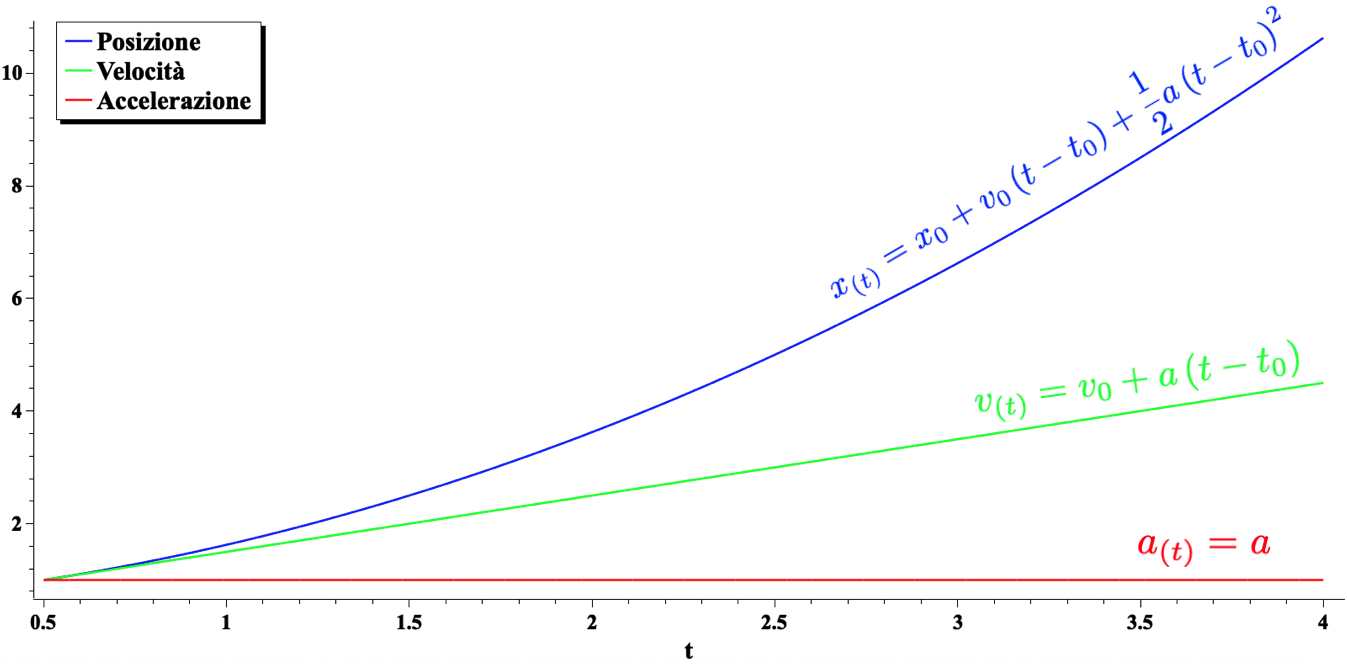
\includegraphics[width=13cm]{images/Motorettunifacc1.png} 
\caption{Un esempio del grafico di accelerazione (rosso), velocità (verde) e posizione (blu), nel moto uniformemente accelerato unidimensionale. L'asse delle ascisse rappresenta il tempo, mentre quello delle ordinate la variabile dipendente.}
\label{default}
\end{center}
\end{figure}




\section{Moto armonico semplice}
Il moto armonico semplice è un tipo di moto, periodico, che avviene in una regione confinata dello spazio.\\
Prendiamo il caso in cui un punto materiale oscilla tra una posizione minima ed una massima, nel caso più generale possibile possiamo scrivere la sua legge oraria utilizzando una funzione armonica.




\begin{equation}
\boxed{x_{(t)} = A\sin\sx \omega t +\phi\dx}
\end{equation}

Dove $A$ è l'ampiezza di oscillazione, il punto si muove tra $ x = -A$ ed $x = A$.\\
$\omega$ è la pulsazione, $\omega = 2\pi\nu$ dove $\nu$ è la frequenza ed indica in numero di oscillazioni effettuate in un secondo. \\
$\phi$ è lo sfasamento iniziale, è collegato alla posizione iniziale tramite: $ x_0 \coloneqq x_{(0)} = A\sin\phi$\\
Una volta nota la legge oraria è immediato calcolare velocità ed accelerazione, dato che basta derivare rispetto al tempo.\\
Introduciamo ora una notazione molto utilizzata in fisica ovvero, l'utilizzo di un punto posto sopra il simbolo di una grandezza per indicarne la derivata totale rispetto al tempo.

\begin{equation}
v_{(t)} = \dot x_{(t)} = A\omega\cos\sx\omega t +\phi\dx
\end{equation}
\begin{equation}
a_{(t)} = \dot v_{(t)} = \ddot x_{(t)} = -A\omega^2\sin\sx\omega t +\phi\dx
\end{equation}
Possiamo notare che esiste una relazione tra accelerazione e posizione.


\subsection{Equazione differenziale dell'oscillatore armonico}
Come si può notare chiaramente, l'accelerazione è direttamente proporzionale alla posizione.


\begin{equation}
\ddot x = -\omega^2x\seg \boxed{\ddot x_{(t)} + \omega^2x_{(t)} = 0}
\end{equation}

La $(1.10)$ è un'equazione differenziale al secondo ordine, a coefficienti costanti, omogenea. Che unita alle due condizioni iniziali: $x_{(0)} = A\sin\phi $ ed $\dot x_{(0)} = A\omega\cos\phi $ ha come soluzione la $(1.7)$.\\
Ora che sappiamo che $a_{(x)} = -\omega^2x$ possiamo utilizzare la formula $(1.5)$ per ottenere $v_{(x)}$.

\begin{equation}
v^2_{(x)} = v_0^2 - \omega^2\sx x^2 - x_0^2\dx
\end{equation}

\begin{figure}[htbp]
\begin{center}
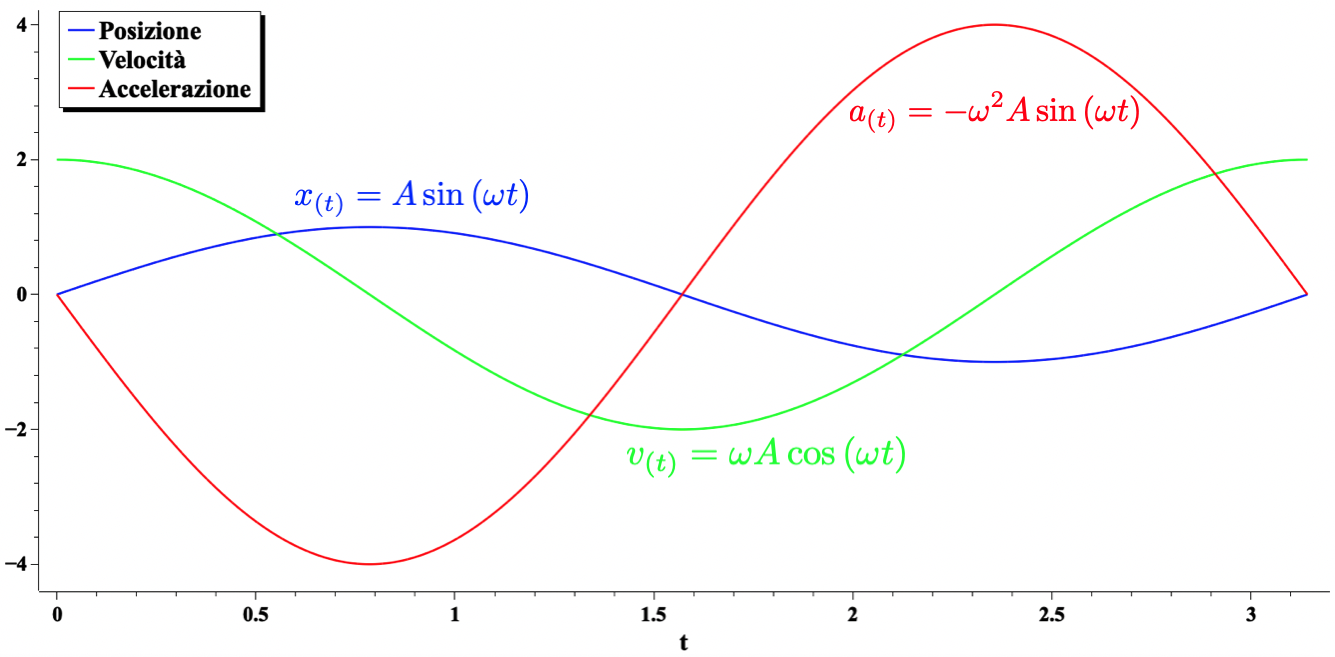
\includegraphics[width=13cm]{images/Motoarm1.png} 
\caption{Un esempio del grafico di accelerazione (rosso), velocità (verde) e posizione (blu), nel moto armonico semplice. L'asse delle ascisse rappresenta il tempo, mentre quello delle ordinate la variabile dipendente.}
\label{default}
\end{center}
\end{figure}




\section{Moto rettilineo smorzato esponenzialmente}
Questo tipo di moto si incontra quando si ha un'accelerazione proporzionale alla velocità con coefficiente negativo (altrimenti sarebbe forzato esponenzialmente nel tempo). Introduciamo quindi un parametro di smorzamento $\beta>0$.




\begin{equation}
a_{(t)} = -\beta v_{(t)} = \dot v_{(t)}\seg \frac{\dot v}{v} = -\beta \seg \int_{t_0}^{t}dt' \frac{\dot v}{v} =  -\beta\int_{t_0}^{t}dt'
\end{equation}

\begin{equation}
\ln{\left[ \frac{v_{(t)}}{v_0}\right]} = -\beta\sx t-t_0\dx\seg \boxed{v_{(t)} = v_0e^{-\beta\sx t-t_0\dx}} = \dot x 
\end{equation}

\begin{equation}
\boxed{x_{(t)} = x_0 + \frac{v_0}\beta\left[1-e^{-\beta\sx t-t_0\dx}\right]}
\end{equation}

\begin{equation}
a = -\beta \cancel{v} = \cancel{v}\frac{dv}{dx}\seg \boxed{v_{(x)} = v_0 - \beta\sx x - x_0\dx}
\end{equation}

\begin{figure}[htbp]
\begin{center}
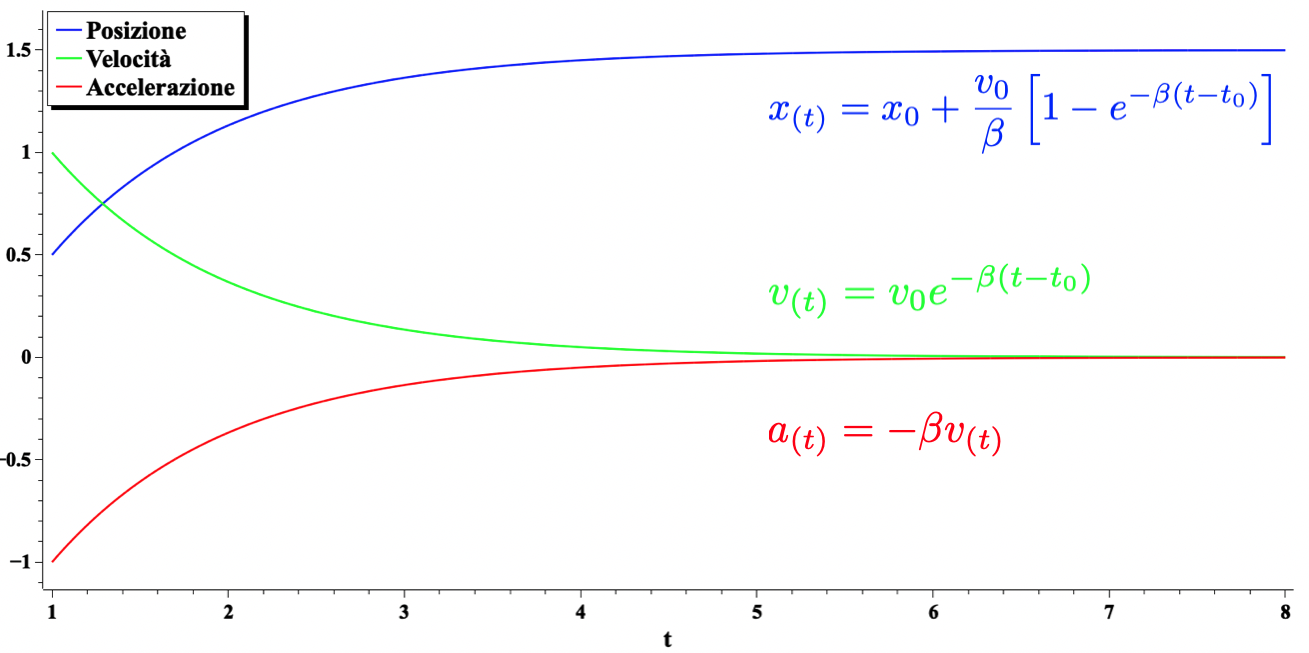
\includegraphics[width=13cm]{images/Motosmorz1.png} 
\caption{Un esempio del grafico di accelerazione (rosso), velocità (verde) e posizione (blu), nel moto smorzato esponenzialmente. L'asse delle ascisse rappresenta il tempo, mentre quello delle ordinate la variabile dipendente.}
\label{default}
\end{center}
\end{figure}




\section{Coordinate curvilinee e coordinate polari nel piano}
In moti casi in fisica risulta particolarmente conveniente utilizzare tipologie diverse di coordinate, rispetto a quelle cartesiane. Due di queste sono le coordinate curvilinee e quelle polari.\\
Le coordinate cartesiane identificano la posizione di un punto materiale mediante tre coordinate, corrispondenti alla proiezione del punto lungo gli assi cartesiani. Utilizzando i versori canonici $\hat\imath$, $\hat\jmath$ e $\hat k$ possiamo scrivere:




\begin{equation}
\vec x = \sx x, y, z\dx = x\hat\imath + y\hat\jmath + z\hat k\seg \vec v = \dot x\hat\imath +\dot y\hat\jmath +\dot z\hat k\quad\quad\vec a = \ddot x\hat\imath +\ddot y\hat\jmath +\ddot z\hat k
\end{equation}

Le coordinate curvilinee identificano come posizione, la distanza effettivamente percorsa dal punto materiale, e utilizzano come direzioni principali quella tangente $(\hat\tau)$ e quella normale $(\hat n)$.\\

\begin{figure}[htbp]
\begin{minipage}[b]{0.47\textwidth}
\centering
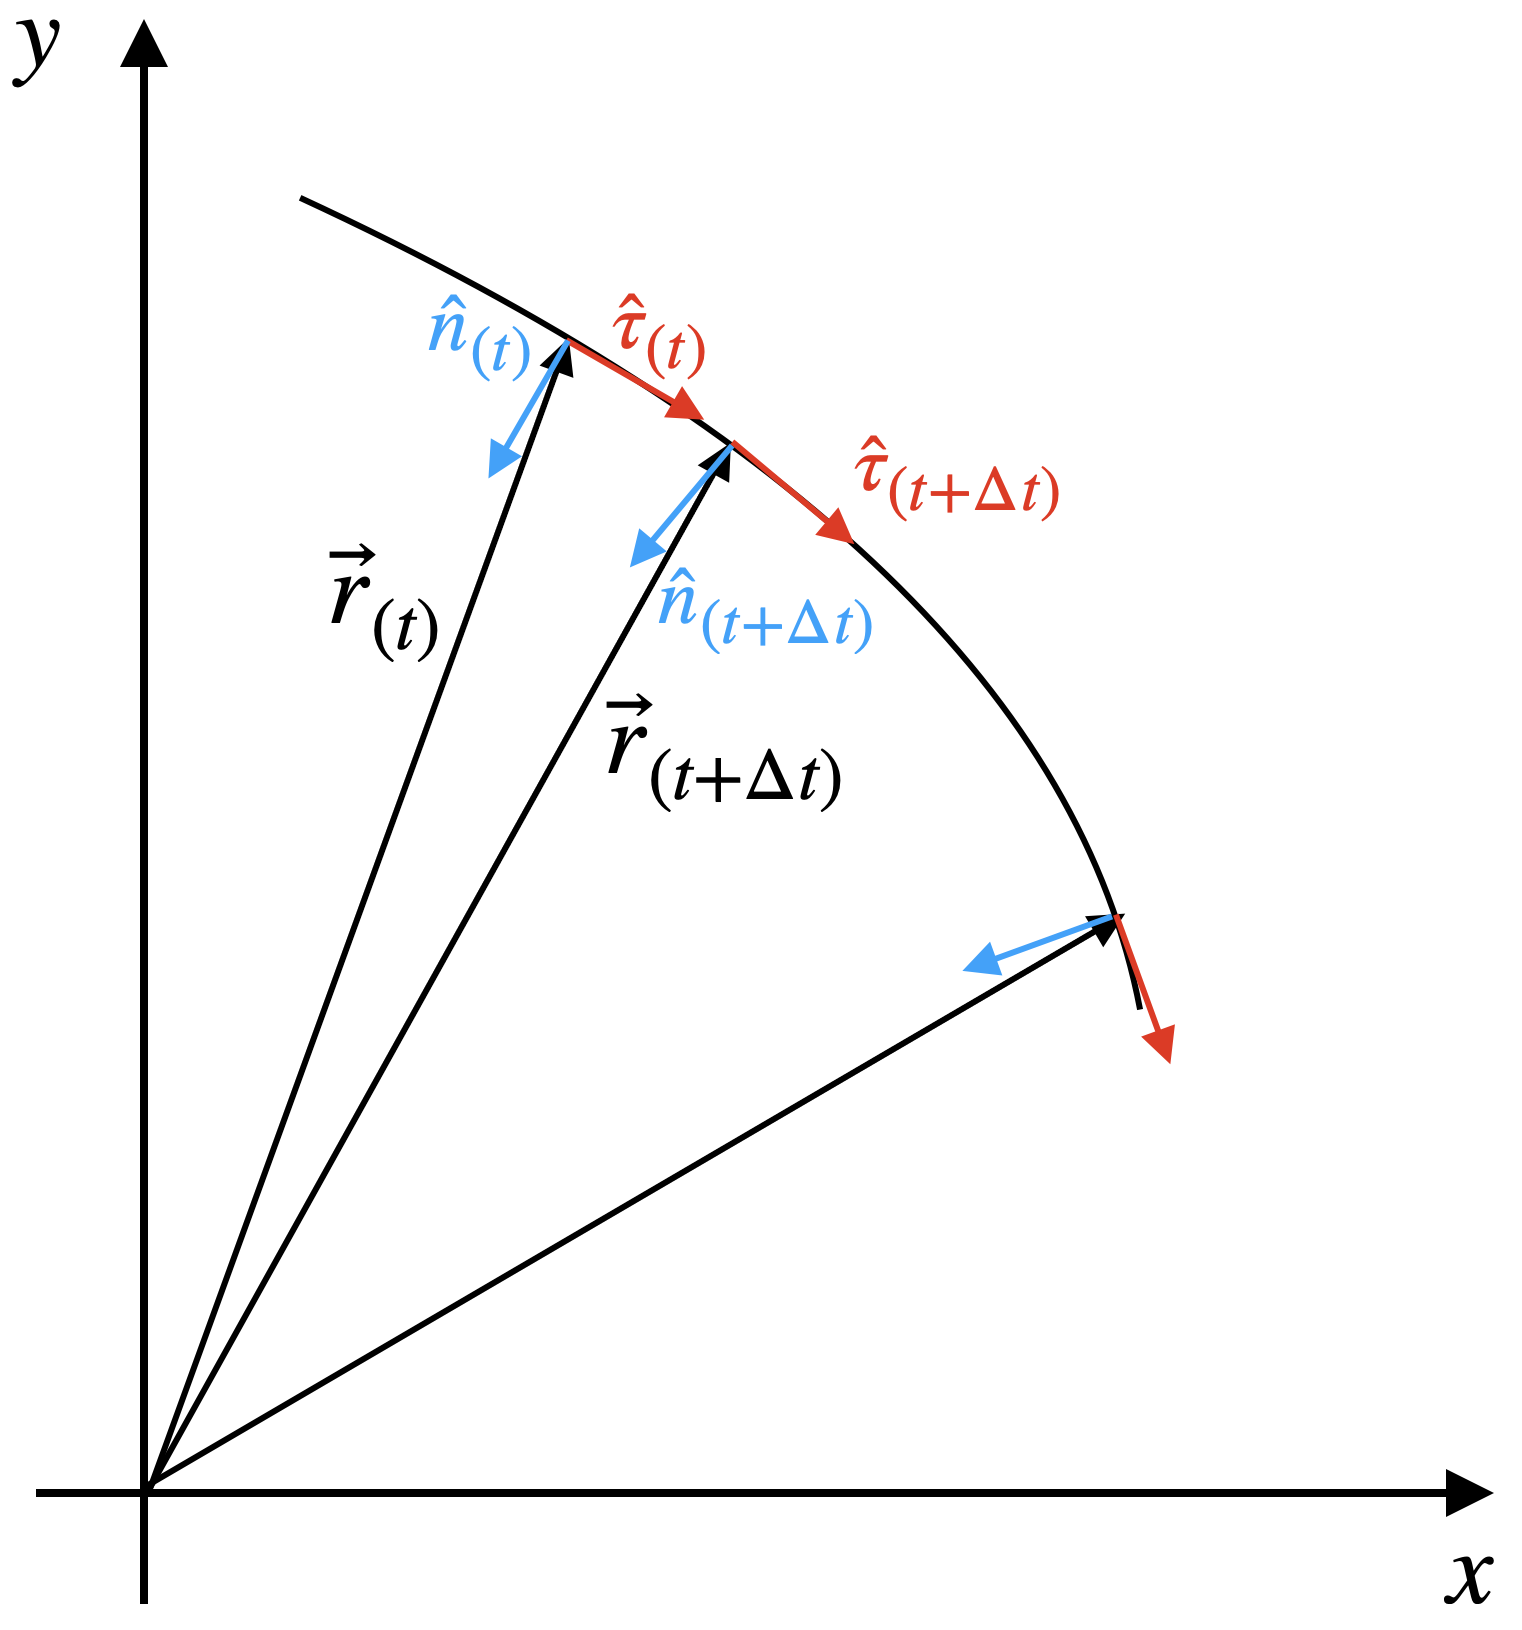
\includegraphics[width=7cm]{images/coordcurv.png}
\caption{Rappresentazione dei versori tangente e normale lungo un tratto di curva.}
\label{etichetta1}
\end{minipage}
\hfill
\begin{minipage}[b]{0.47\textwidth}
\centering
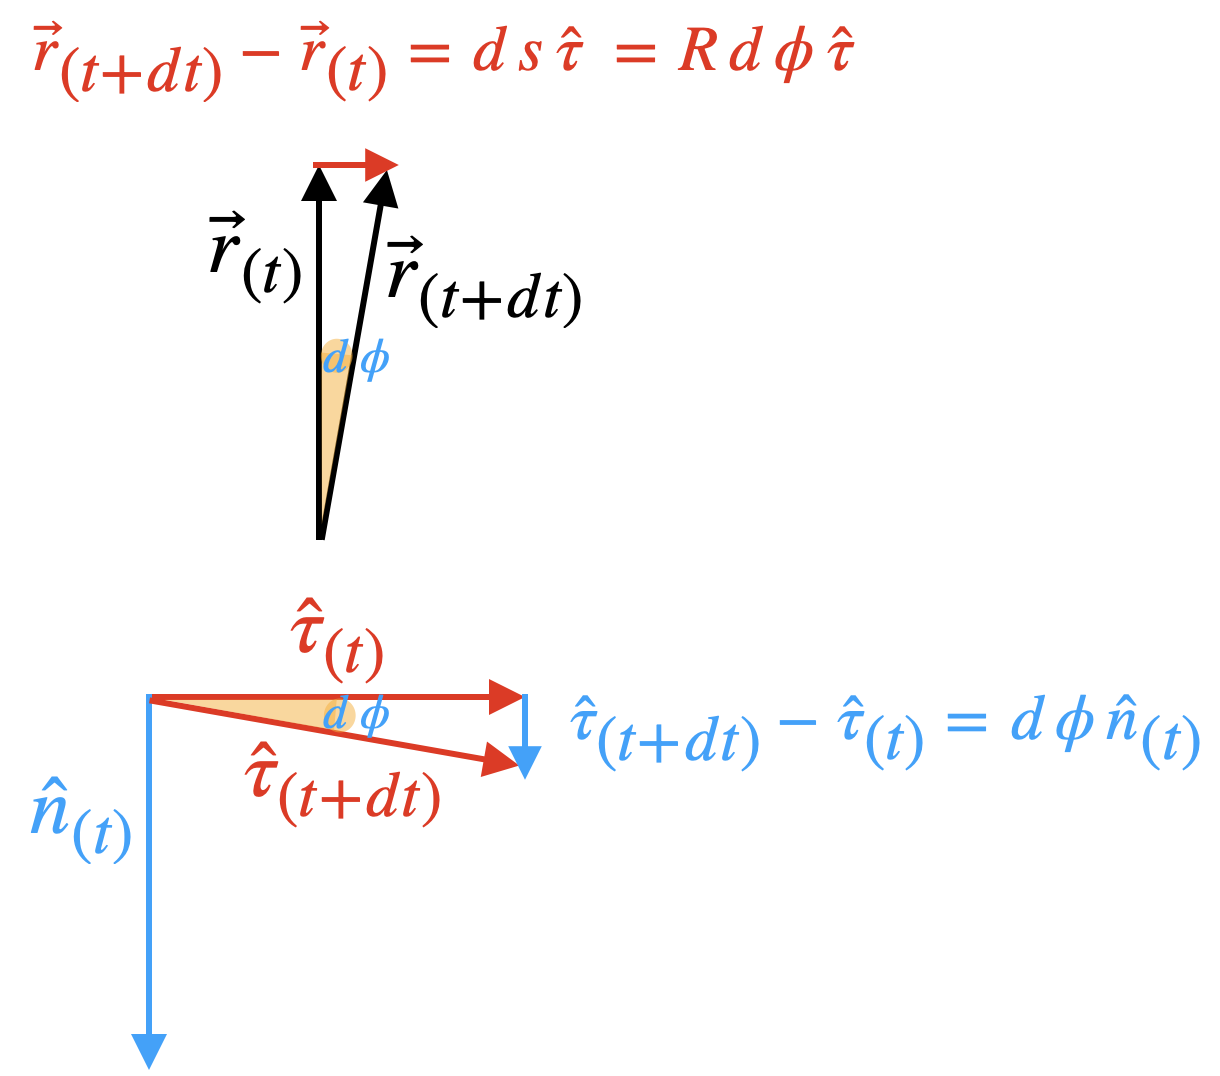
\includegraphics[width=7cm]{images/drdtau.png}
\caption{Rappresentazione grafica della variazione infinitesima del vettore $\vec r$ e del versore $\hat\tau$.}
\label{etichetta2}
\end{minipage}
\hfill
\end{figure}

\newpage


\begin{equation}
d\vec x = ds\hat\tau\seg \vec v = \dot s \hat\tau = v\hat\tau\seg \vec a = \ddot s\hat\tau + \dot s\dot\phi\hat n
\end{equation}

\begin{equation}
\dot\phi = \frac{d\phi}{ds}\dot s = \dot s \frac{d\phi}{Rd\phi} = \frac{v}{R}
\end{equation}

\begin{equation}
\boxed{\vec v = v\hat\tau}\quad\quad \boxed{\vec a = \dot v \hat\tau + \frac{v^2}{R}\hat n = a_t\hat\tau + a_n\hat n}
\end{equation}
                                                                                                                                                                                                                                                                                                                                                                                                                                                                                                                                                                                                                                                                                                                                                                                                                                                                                                                                                                                                                                                                                                                                                                                                                                                                                                                                                                                                                                                                                                                                                                                                                                                                                                                                                                                                                                                                                                                                                                                                                                                                                                                                                                                                                                                                                                                                                                                                                                                                                                                                                                                                                                                                                                                                                                                                                                                                                                                                                                                                                                                                                                                                                                                                                                                                                                                                                                                                                                                                                                                                                                                                                                                                                                                                                                                                                                                                                                                                                                                                                                                                                                                                                                                                                                                                                                                                                                                                                                                                                                                                                                                                                                                                                                                                                                                                                                                                                                                                                                                                                                                                                                                                                                                                                                                                                                                                                                                                                                                                                                                                                                                                                                                                                                                                                                                                                                                                                                                                                                                                                                                                                                                                                                                                                                                                                                                                                                                                                                                                                                                                                                                                                                                                                                                                             
L'accelerazione in coordinate curvilinee ha due componenti, una tangente ed una normale o centripeta. La velocità invece è sempre tangente alla traiettoria percorsa.\\
Per quanto riguarda invece le coordinate polari, si scelgono come direzioni principali quella radiale $(\hat r)$ e quella trasversa $(\hat\phi)$.

\begin{figure}[htbp]
\centering
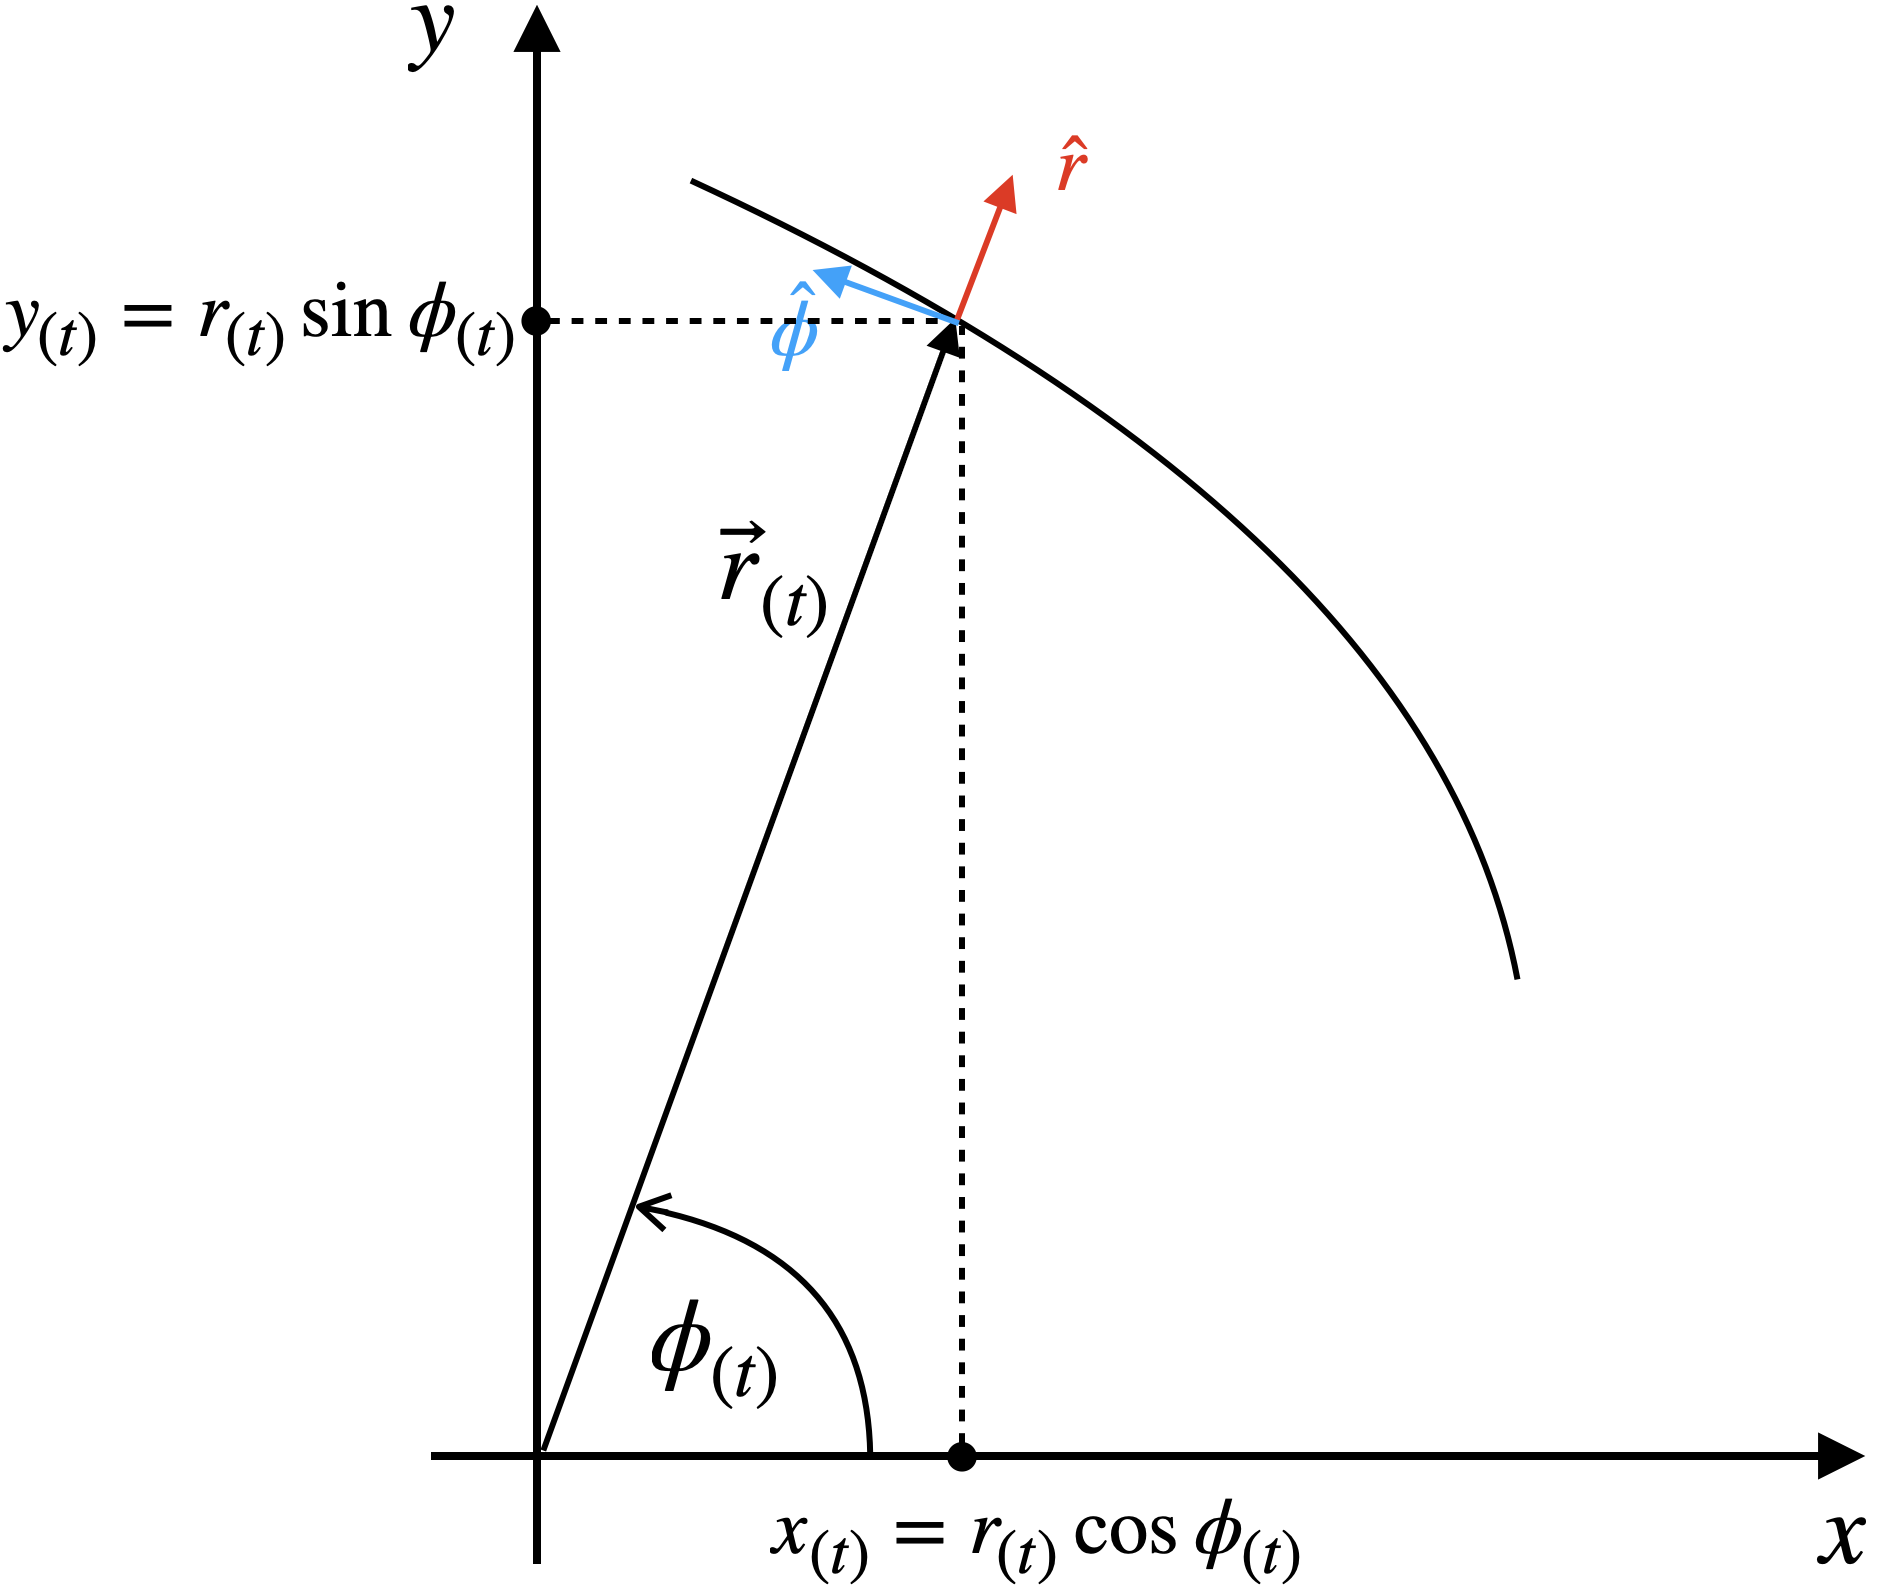
\includegraphics[width=7cm]{images/coordpol.png}
\caption{Rappresentazione dei versori tangente e normale lungo un tratto di curva.}
\label{etichetta1}
\end{figure}


\begin{equation}
\boxed{\vec x = r\hat r} \seg \boxed{\vec v = \dot r \hat r + r\dot\phi\hat\phi}
\end{equation}

Per ottenere l'espressione dell'accelerazione in coordinate polari è necessario svolgere alcuni calcoli.

\begin{equation}
\vec a = \frac{d\vec v}{dt} = \frac{d}{dt}\sx \dot r \hat r + r\dot\phi\hat\phi \dx = \ddot r\hat r + \dot r\frac{d\hat r}{dt} + \dot r \dot \phi \hat\phi + r\ddot\phi\hat\phi + r\dot\phi\frac{d\hat \phi}{dt}
\end{equation}

\begin{equation}
\frac{d\hat r}{dt} = \dot\phi\hat\phi\quad\quad\quad \frac{d\hat \phi}{dt} = -\dot\phi\hat r
\end{equation}

\begin{equation}
\vec a = \sx \ddot r - r\dot\phi^2\dx\hat r + \sx 2\dot r\dot\phi + r\ddot\phi\dx\hat\phi
\end{equation}
$$\Downarrow$$

\begin{equation}
\boxed{\vec a = \sx \ddot r - r\dot\phi^2\dx\hat r + \left[\frac{1}{r}\frac{d}{dt} \sx r^2\dot\phi\dx\right]\hat\phi = a_r\hat r + a_{\phi}\hat\phi}
\end{equation}




\section{Moto circolare uniforme}
Un moto circolare è un moto planare in cui il punto materiale descrive come traiettoria una circonferenza. Esso può essere scomposto in due moti armonici. Il moto circolare uniforme è chiamato in questo modo perché avviene a velocità angolare $(\omega)$ costante.
Usiamo come coordinate principali quelle curvilinee.




\begin{equation}
s_{(t)} = R\phi_{(t)}\seg \phi = \frac sR\seg \omega = \dot \phi = \frac vR
\end{equation}
 
 Otteniamo la relazione:
\begin{equation}
\boxed{v = \omega R}
\end{equation}
 Ora esattamente come abbiamo fatto nel paragrafo $(1.1)$ calcoliamo la legge oraria per la variabile $\phi$.
 
\begin{equation}
\omega_{(t)} = \dot\phi \seg \phi_{(t)} = \phi_0 + \int_{t_0}^{t}dt'\omega_{(t')}\quad\quad \omega_{(t)} = \omega_0
\end{equation}
\begin{equation}
\boxed{\phi_{(t)} = \phi_0 +\omega_0\sx t - t_0\dx}
\end{equation}

\begin{equation}
v = \omega_0R\seg a = a_n = \frac{v^2}R = \omega_0^2R
\end{equation}

Il periodo di rotazione è:
\begin{equation}
T = \frac1\nu = \frac{2\pi}{\omega_0} = \frac{2\pi R}v
\end{equation}




\section{Moto circolare uniformemente accelerato}
Il moto circolare non uniforme si ha quando la velocità angolare non è costante nel tempo. Questo comporta che la componente tangente di $\vec a$ non è nulla. Nel caso in cui $\omega$ è lineare nel tempo si avrà un moto circolare uniformemente accelerato.
\\ Definiamo quindi l'accelerazione angolare:




\begin{equation}
\alpha_{(t)} = \dot \omega = \ddot \phi\seg a_t = \dot v = \frac d{dt}\sx \omega R\dx = \alpha R
\end{equation}

Di conseguenza avremo che:

\begin{equation}
\omega_{(t)} = \omega_0 + \int_{t_0}^tdt'\alpha_{(t')}  = \omega_0 + \alpha_0\sx t - t_0\dx \seg
\phi_{(t)} = \phi_0 + \omega_0\sx t - t_0\dx+ \frac12\alpha_0\sx t - t_0\dx^2
\end{equation}


Esiste anche un analogo della formula $(1.6)$.

\begin{equation}
\alpha =\dot \omega = \frac{d\omega}{d\phi}\dot\phi\seg \omega^2_{(\phi)} = \omega_0^2 + 2\alpha_0\sx\phi-\phi_0\dx
\end{equation}

Utilizzando un formalismo vettoriale possiamo scrivere che:
\begin{figure}[htbp]
\centering
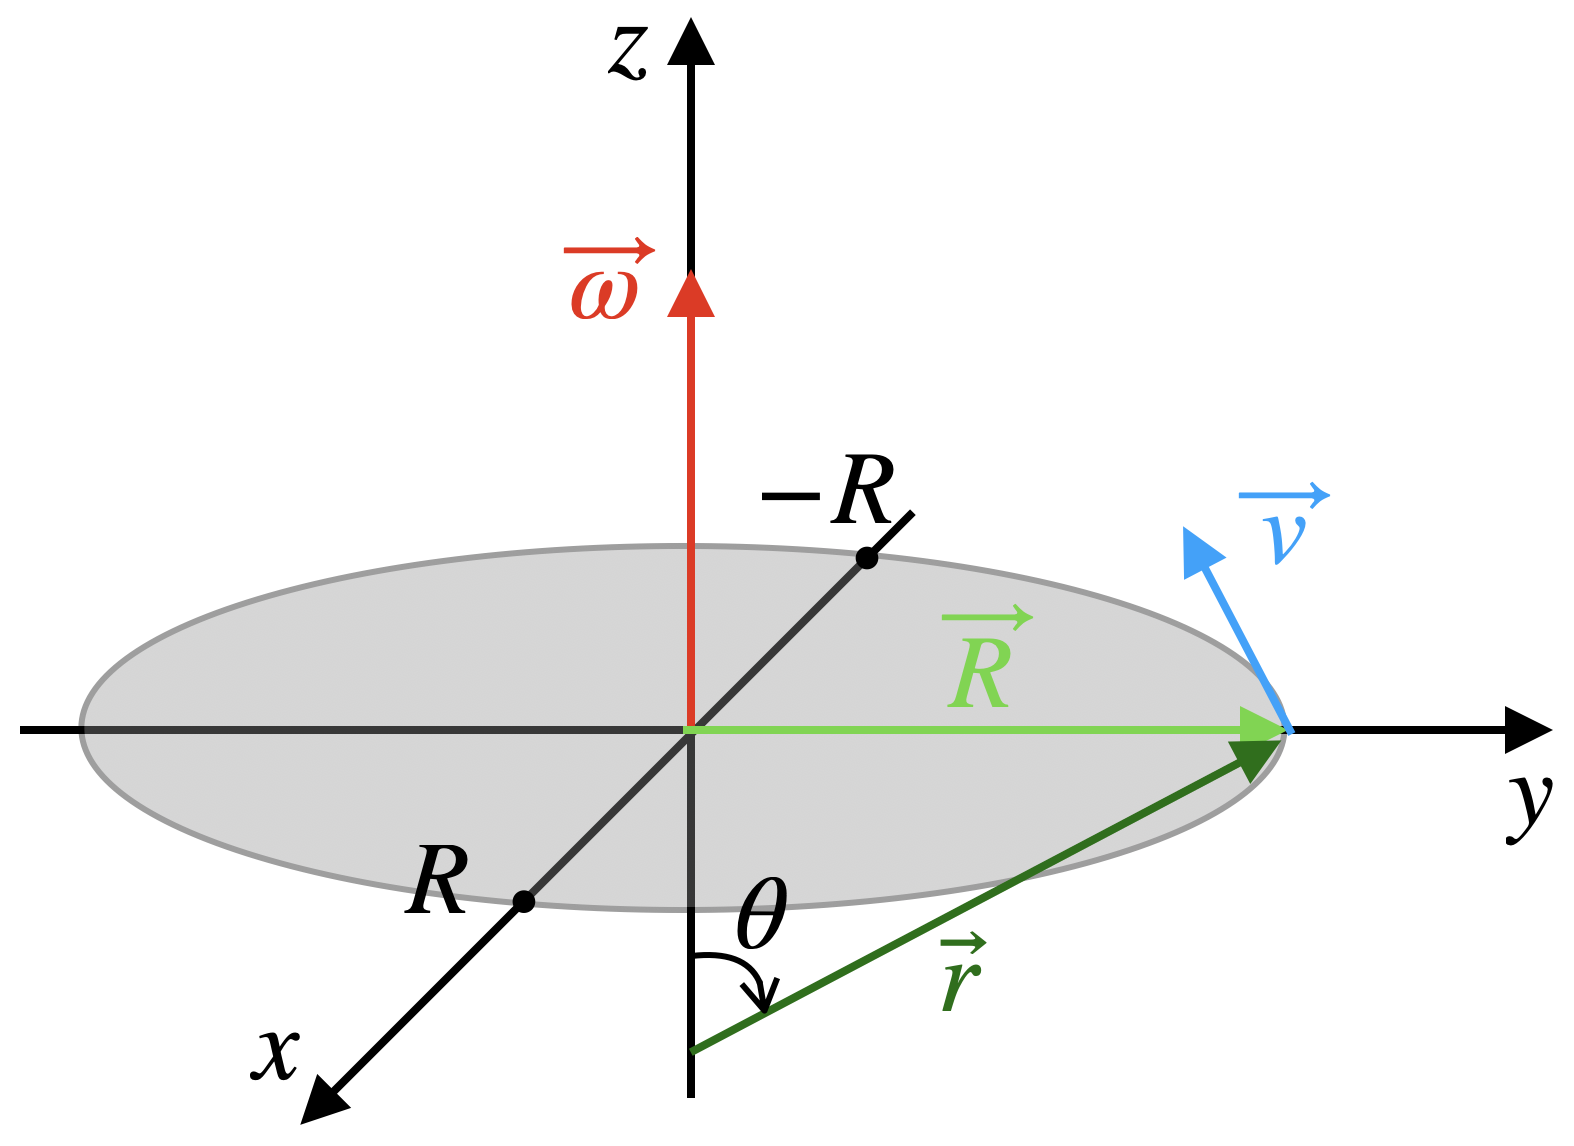
\includegraphics[width=7cm]{images/ovetr.png}
\caption{Schema di un moto circolare con la rappresentazione del vettore velocità angolare.}
\label{etichetta1}
\end{figure}

\begin{equation}
\vec v = \vec\omega\times\vec R\seg \left| \vec v \right|  = \omega R
\end{equation}
Se trasliamo verso il l'origine degli assi otteniamo che:
\begin{equation}
\vec v = \vec\omega\times\vec r\seg \left| \vec v \right|  = \omega r\sin\theta = \omega R
\end{equation}

Ne segue che dato un vettore generico rotante $\vec A$ avremo che:
\begin{equation}
\frac{d\vec A}{dt} = \vec\omega\times\vec A
\end{equation}

Infine scriviamo la forma dell'accelerazione.
\begin{equation}
\vec a = \frac d{dt}\sx\vec\omega\times\vec r\dx = \vec \alpha\times \vec r + \vec\omega\times\vec v
\end{equation}

Come possiamo notare se consideriamo il caso particolare in cui $\alpha = 0 $ otteniamo:
\begin{equation}
\vec a = \vec \omega\times\vec v = \vec \omega\times\sx \vec\omega\times \vec R\dx = \sx\cancel{\vec\omega\cdot\vec R}\dx\vec\omega - \omega^2\vec R = \omega^2R\hat n = \frac{v^2}R\hat n
\end{equation}

Possiamo decomporre il moto circolare in due moti armonici, uno per l'asse $x$ ed uno per l'asse $y$.

\begin{equation}
\begin{cases}
x_{(t)} = R\cos\phi_{(t)}\\
y_{(t)} = R\sin\phi_{(t)}\\
\end{cases}\seg
\begin{cases}
\dot x_{(t)} = -R\dot\phi\sin\phi_{(t)}\\
\dot y_{(t)} = R\dot\phi\cos\phi_{(t)}\\
\end{cases}
\end{equation}

\begin{figure}[htbp]
\centering
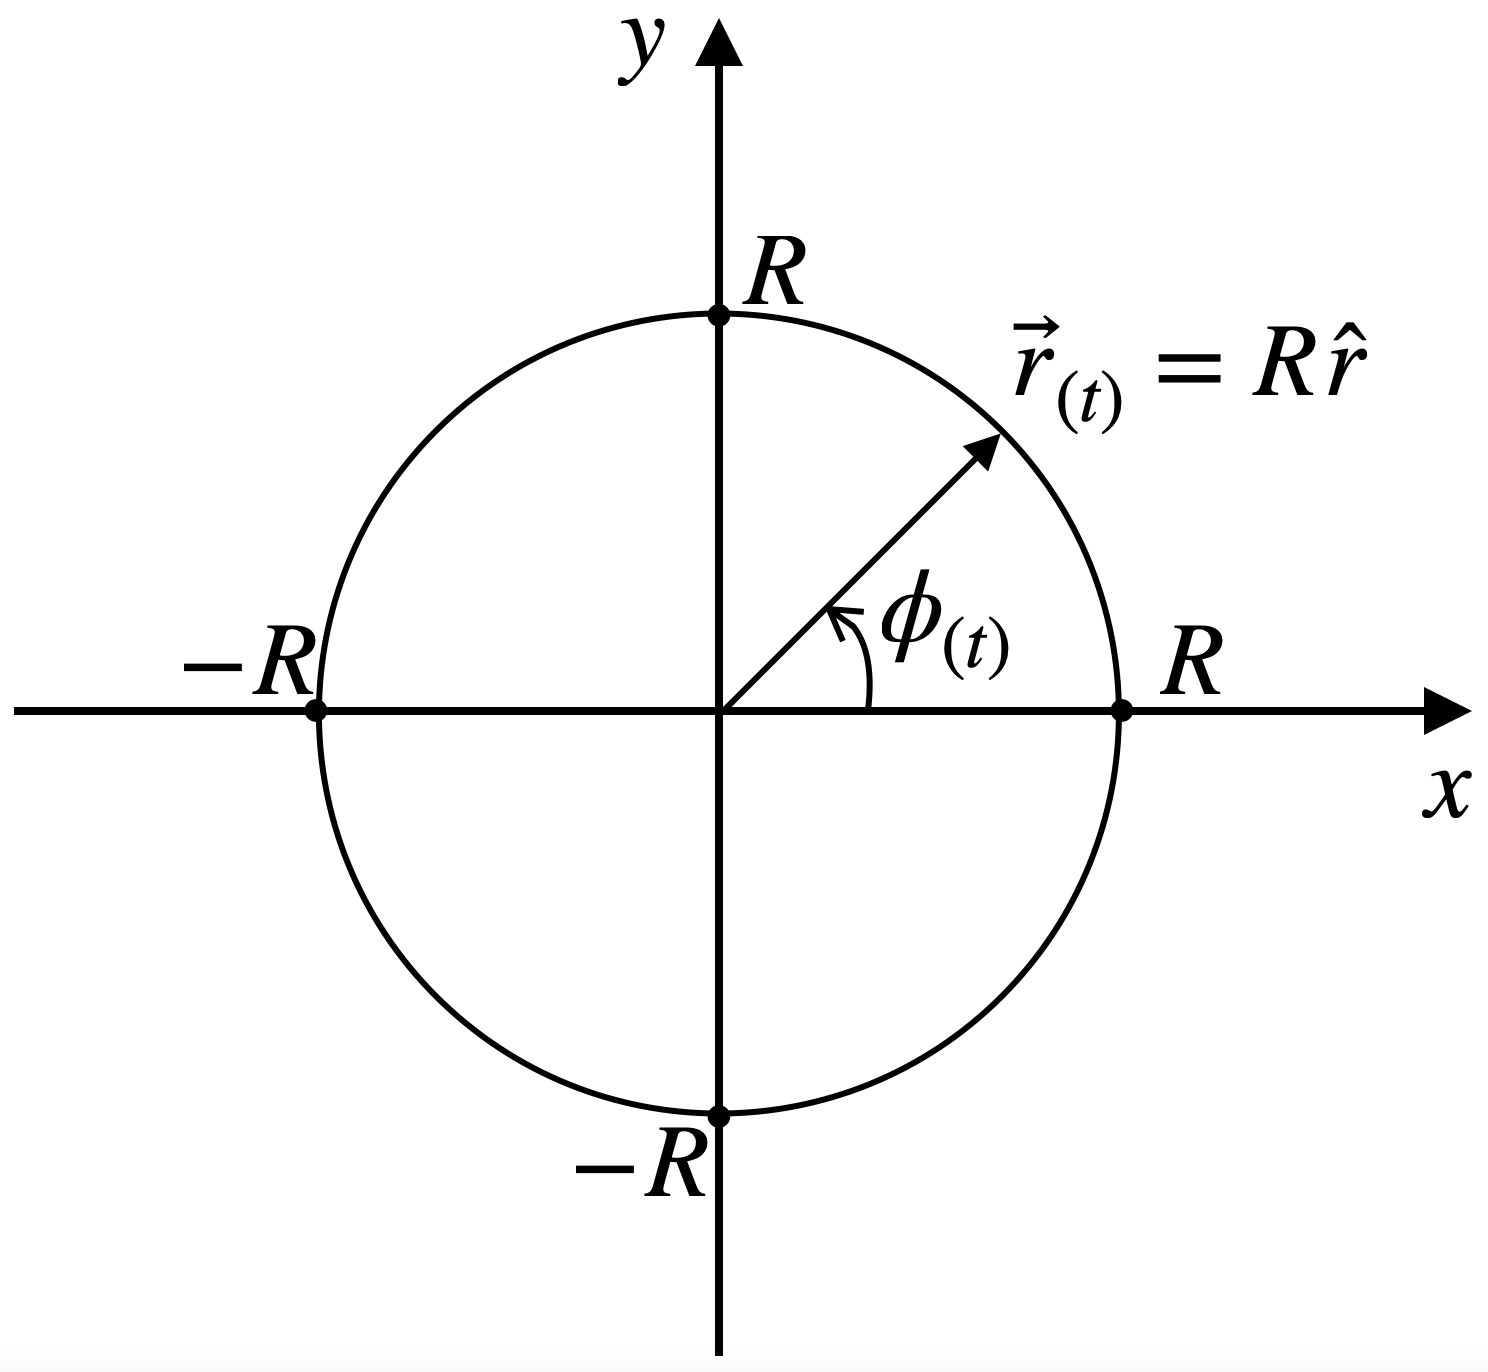
\includegraphics[width=7cm]{images/circ.png}
\caption{Rappresentazione della traiettoria, del raggio vettore e della variabile angolare $\phi$ nel moto circolare.}
\label{etichetta1}
\end{figure}




\section{Moto parabolico}
Un moto parabolico è il moto che compie un proiettile lanciato con una certa velocità $\vec v_0$, sottoposto ad un campo di forze uniforme e costante, ovvero il campo gravitazionale in prossimità della superficie terrestre.\\
Il moto parabolico può essere scomposto in due moti disaccoppiati, un moto rettilineo uniforme lungo l'asse $x$ ed un moto rettilineo uniformemente accelerato lungo l'asse $y$. Questo perché non sono presenti forze orizzontali, e l'unica forza agente sul corpo è quella gravitazionale in direzione verticale. Dunque è presente un'accelerazione pari a: $\vec a = -g\hat\jmath $. Per semplicità poniamo l'istante iniziale $ t_0 = 0$.




\begin{equation}
\begin{cases}
x_{(t)} = x_0 + v_0\cos\phi t\\
y_{(t)} = y_0 + v_0\sin\phi t - \frac12 g t^2
\end{cases}\seg
\begin{cases}
\dot x_{(t)} = v_0\cos\phi \\
\dot y_{(t)} = v_0\sin\phi - gt
\end{cases}
\end{equation}

Si può anche ricavare l'equazione della traiettoria, isolando il tempo dalla legge oraria per $x$ ed inserendolo nell'equazione per $y$.

\begin{equation}
t = \frac{x-x_0}{v_0\cos\phi}\seg y_{(x)} = y_0 + \tan\phi\sx x-x_0\dx-\frac{g}{2v_0^2\cos^2\phi}\sx x-x_0\dx^2
\end{equation}
 Come si può notare è l'equazione di una parabola centrata in $x_0$ con coefficiente del termine di secondo grado sempre negativo, stante ad indicare che la traiettoria parabolica ha sempre la concavità rivolta verso il basso, come è giusto che sia dato che il punto materiale dovrà cadere a terra.\\ Imponendo la $y$ uguale a zero, possiamo ricavare il tempo di volo.
 
\begin{equation}
y_0 + v_0\sin\phi \tau - \frac12 g \tau^2 = 0 \seg \boxed{\tau = \frac{v_0}{g}\sin\phi + \sqrt{\frac{v_0^2}{g^2}\sin^2\phi+2\frac{y_0}g}}
\end{equation}

 Calcolando $x_{(\tau)}$ oppure imponendo uguale a zero $y_{(x)}$, otterremo la gittata del proiettile, ovvero la massima distanza percorsa lungo l'asse orizzontale.

\begin{equation}
\boxed{R = x_0 + \frac{v_0^2}{g}\sin\sx\phi\dx\cos\sx\phi\dx + v_0\cos\phi\sqrt{\frac{v_0^2}{g^2}\sin^2\phi+2\frac{y_0}g}}
\end{equation}

Se consideriamo il caso in cui il proiettile parte da terra, abbiamo che $y_0 = 0$ quindi la gittata diventerà:

\begin{equation}
R = x_0 +2\frac{v_0^2}{g}\sin\sx\phi\dx\cos\sx\phi\dx = x_0 + \frac{v_0^2}{g}\sin\sx2\phi\dx
\end{equation}
Il valore massimo di questa $R$ si ottiene quando il $\sin\sx2\phi\dx$ è pari ad 1, dunque la gittata massima si otterrà per $\phi = 45^\circ$. Dobbiamo ricordare che nel caso in cui $x_0\ne0$, $R$ rappresenta ovviamente l'ascissa del punto in cui il proiettile cade a terra. Quindi per calcolare la distanza effettivamente percorsa, si deve considerare la differenza $R-x_0$.

Per quanto riguarda invece la quota massima raggiunta dal proiettile, bisogna annullare la $\dot y_{(t)}$ per ricavare il tempo in cui si raggiunge tale quota (velocità verticale nulla). 

\begin{equation}
t^* = \frac{v_0}{g}\sin\phi\seg\boxed{h = y_0 + \frac{v_0^2}{2g}\sin^2\phi}
\end{equation}

\begin{figure}[htbp]
\begin{center}
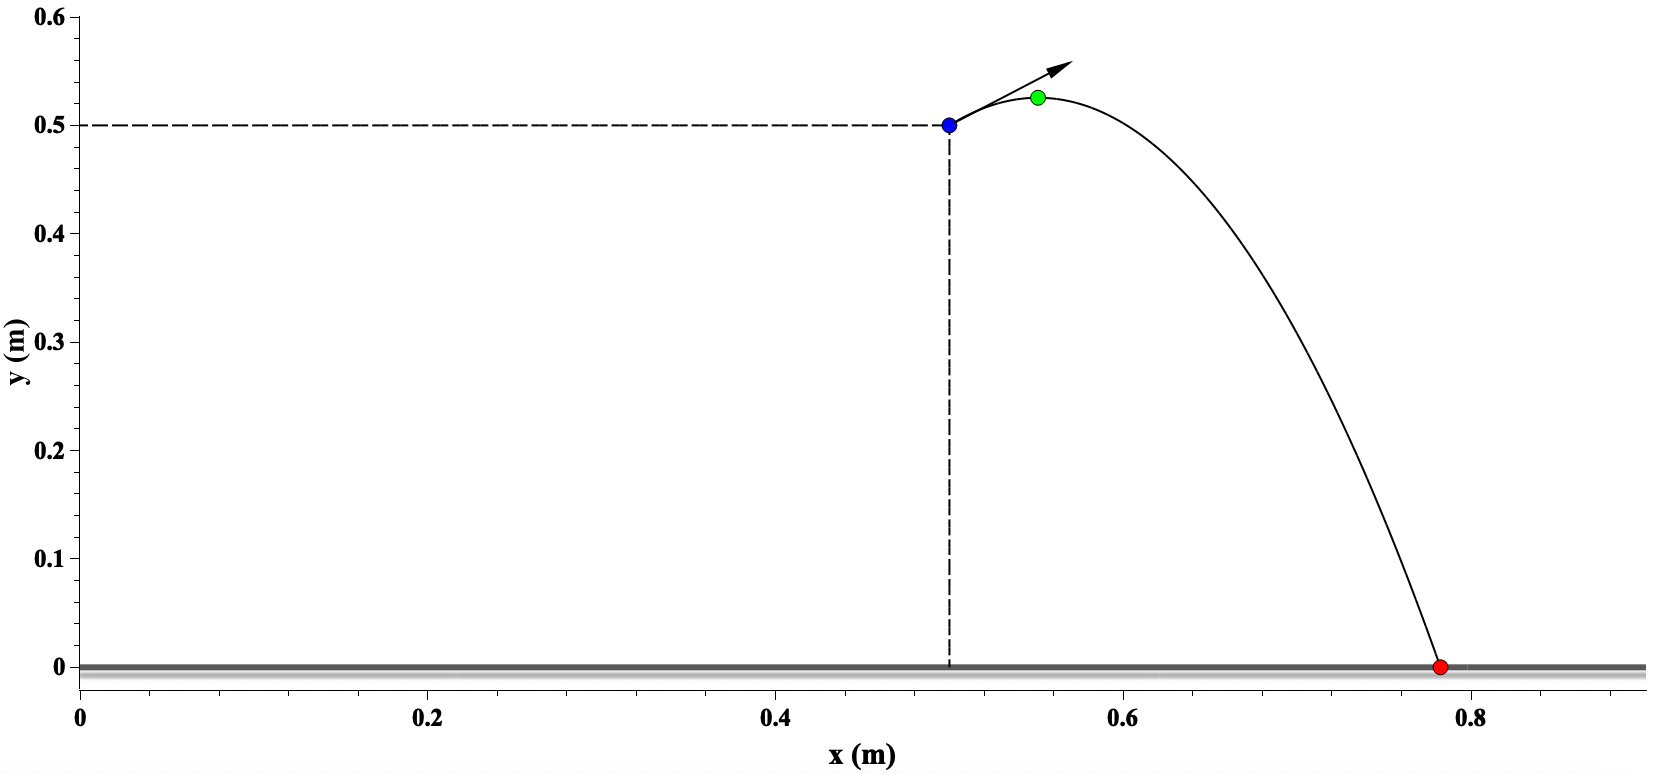
\includegraphics[width=13cm]{images/Motopar1.png} 
\caption{Esmpio di una traiettoria di un moto parabolico generico. Sono stati riportati Il punto iniziale in blu, il punto a quota massima in verde ed il punto ad ascissa massima.}
\label{default}
\end{center}
\end{figure}

\line(1,0){500}
%-----------------------------------------------------------------------------------------------------------------------------------
\chapter{Dinamica del punto materiale}
%-----------------------------------------------------------------------------------------------------------------------------------



\section{Leggi di Newton}




\begin{enumerate}
\item Prima legge di Newton (Principio d'inerzia): Un corpo non soggetto a forze esterne non subisce cambiamenti di velocità, ovvero resta in quiete o in moto rettilineo uniforme.
\item Seconda legge di Newton: La somma delle forze che agiscono su un corpo è proporzionale all'accelerazione del corpo stesso, mediante un coefficiente chiamato massa inerziale.\\
\begin{equation}
\boxed{\vec F = m\vec a}
\end{equation}
\item Terza legge di Newton (Principio di azione e reazione): Se un corpo $A$ esercita una forza $F$ su un corpo $B$, allora $B$ esercita una forza $-F$ su $A$.
Quindi la forza ha le unità di misura di una massa per una lunghezza per un tempo alla meno due.

\end{enumerate}

L'unità di misura della forza è il Newton $(N)$ ed è definito come $\sx Kg\frac m{s^2}\dx$. 
$$ \vec F = m\vec a = m\frac{d\vec v}{dt} = m\frac{d^2\vec x}{dt^2}\quad\quad \left[F\right] = M\cdot L\cdot T^{-2} \seg 1N \coloneqq 1 Kg\cdot\frac m{s^2}$$




\section{Quantità di moto}
Una grandezza molto importante che si introduce in dinamica è la quantità di moto o impulso o momento (lineare). La quantità di moto di un corpo è definita come il prodotto tra la sua massa e la sua velocità, dunque nel sistema internazionale si misura in chilogrammi per metro al secondo. 




\begin{equation}
\boxed{\vec p = m\vec v}\quad\quad \sss p\ddd = M\cdot L\cdot T^{-1}
\end{equation}

Nel caso in cui la massa dell'oggetto sia costante nel tempo, ovvero nella maggior parte dei casi che incontreremo, derivando l'impulso rispetto al tempo otterremo che:

\begin{equation}
\frac{d\vec p}{dt} = \frac d{dt}\sx m\vec v\dx = m\frac{d\vec v}{dt} = \vec F
\end{equation}

Quindi la seconda legge di Newton nel caso più generale, identifica la forza come la derivata temporale della quantità di moto.

\begin{equation}
\boxed{\vec F = \frac{d\vec p}{dt}}
\end{equation}




\section{Teorema dell'impulso}
Integrando l'equazione $(2.4)$ possiamo ricavare la variazione della quantità di moto tra istante finale e istante iniziale che chiameremo impulso $(\vec J)$.




\begin{equation}
\vec F = \frac{d\vec p}{dt}\seg \int_{t_0}^tdt'\frac{d\vec p}{dt'} = \int_{t_0}^tdt'\vec F\seg \vec p_{(t)} - \vec p_{\sx t_0\dx} = \int_{t_0}^tdt'\vec F
\end{equation}

\begin{equation}
\boxed{\vec J = \int_{t_0}^tdt'\vec F}
\end{equation}

Per il teorema della media, il valor medio della forza  è proprio il rapporto tra variazione di quantità di moto e intervallo di tempo.

\begin{equation}
\vec F_m = \frac1{t-t_0}\int_{t_0}^tdt'\vec F = \frac{\Delta\vec p}{\Delta t}
\end{equation}

\begin{itemize}
\item Se $\vec F$ è costante nel tempo allora:

\begin{equation}
\vec J = \vec F\Delta t\seg \Delta \vec p = \vec J \seg \Delta \vec v =\frac{\vec J}m
\end{equation}
\\
\item Se $\vec F$ è nulla allora:

\begin{equation}
\Delta\vec p = 0 \seg \vec p_{(t)} = cost
\end{equation}
In assenza di forze applicate la quantità di moto di un corpo si conserva.
\end{itemize}




\section{Condizione di equilibrio statico}
Se su un corpo agiscono più forze, diremo che il corpo è in equilibrio statico se e solo se la risultante delle forze (la somma) è nulla.\\ Supponiamo di avere un corpo soggetto ad $n$ forze, se chiamiamo la forza $i$-esima: $\vec F_i$, la risultante sarà:




\begin{equation}
\vec F = \sum_{i=1}^n\vec F_i =  \sum_{i=1}^n m\vec a_i = m \sum_{i=1}^n \vec a_i\quad\mbox{eq. statico}\quad\Leftrightarrow \quad\vec F = \vec 0
\end{equation}




\section{Forza di reazione vincolare}
Ogni volta che un corpo soggetto ad una forza incontra un vincolo, quest'ultimo esercita per il principio di azione e reazione un forza uguale e opposta, in modo tale da bilanciare la forza applicata. La forza di reazione vincolare è chiamata anche forza di reazione normale, dato che è ortogonale al vincolo ed infatti è indicata con la lettera $\vec N$.




\begin{figure}[htbp]
\begin{center}
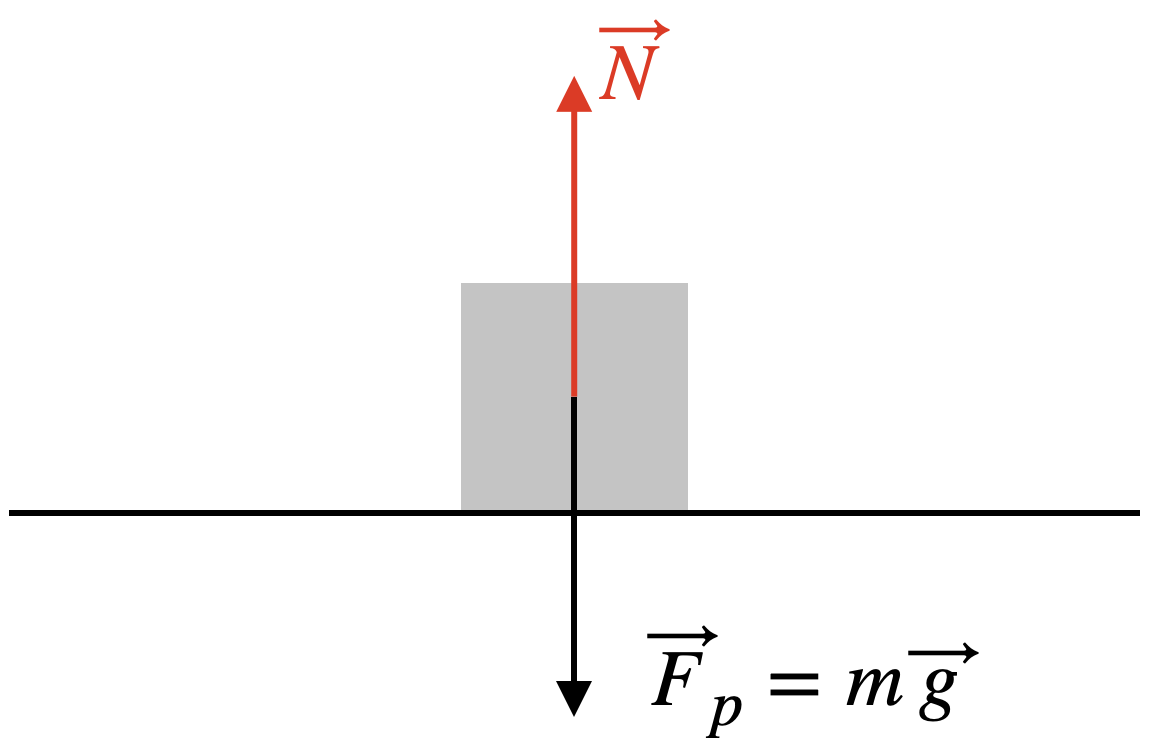
\includegraphics[width=7cm]{images/NP.png}
\caption{Corpo in equilibrio soggetto alla forza peso ed  alla reazione vincolare.}
\label{default}
\end{center}
\end{figure}

In questo caso abbiamo solo due forze, la forza peso e la forza di reazione vincolare e sono entrambe dirette lungo la stessa direzione, ma di verso opposto.

\begin{equation}
\vec N + \vec F_p = \vec 0 \seg N - F_p = N - mg = 0 \seg \boxed{N = mg}
\end{equation}

\begin{figure}[htbp]
\begin{center}
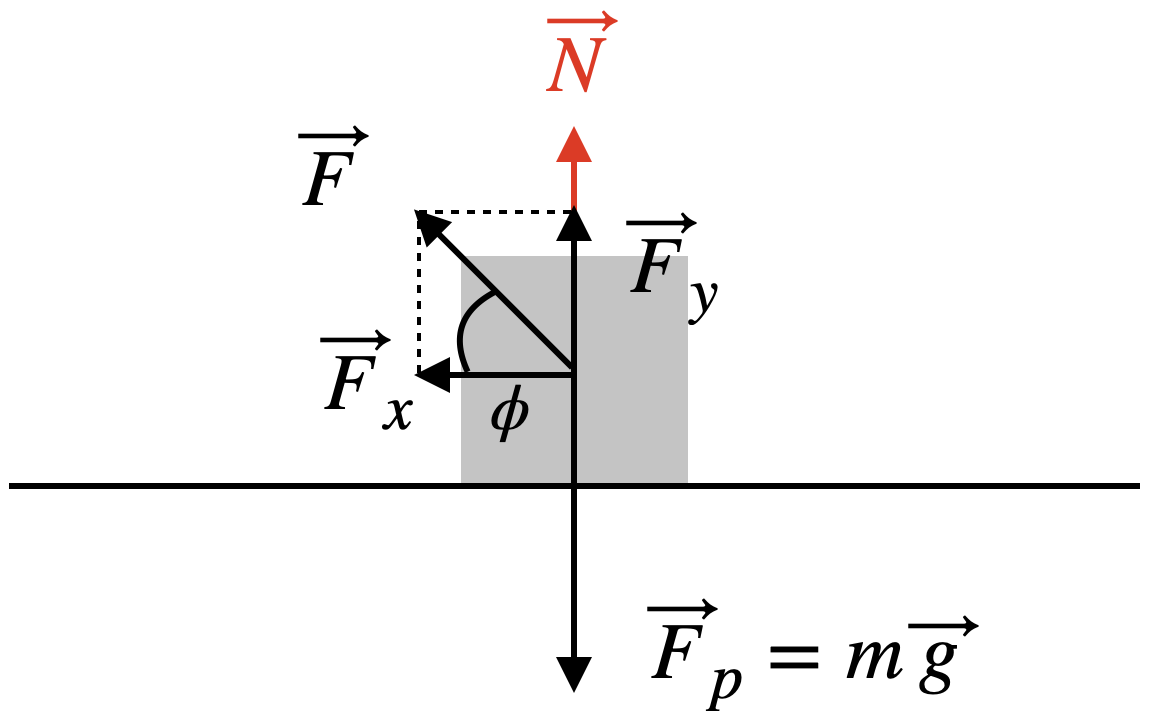
\includegraphics[width=7cm]{images/NPF.png}
\caption{Corpo soggetto alla forza peso, alla forza $\vec F$ ed alla reazione vincolare.}
\label{default}
\end{center}
\end{figure}

Nella situazione rappresentata in figura $(2.2)$, notiamo che l'aggiunta di una terza forza nel sistema modifica l'intensità di $\vec N$. Per prima cosa bisogna scomporre lungo l'asse $x$ ed $y$ la forza $\vec F$.

\begin{equation}
\vec F = \vec F_x + \vec F_y = F_x\hat\imath + F_y\hat\jmath\seg 
\begin{cases}
F_x = -F\cos\phi <0\\
F_y = F\sin\phi>0
\end{cases}
\end{equation}

Adesso procediamo con il calcolo scrivendo le equazioni di Newton.

\begin{equation}
x:\quad\quad F_x = m\ddot x
\end{equation}
\begin{equation}
y:\quad\quad N-mg+F_y = m\ddot y = 0
\end{equation}

\begin{equation}
\mbox{Ne segue che la reazione vincolare è:}\quad \boxed{N = mg -F\sin\phi}
\end{equation}

Per quanto riguarda l'asse $x$, c'è solo la componente orizzontale di $\vec F$ che agisce sul corpo, dunque, supponendo $\phi$ ed il modulo della forza $F$ costanti nel tempo e $\phi\ne\frac\pi2$, il corpo si muove di moto uniformemente accelerato lungo la direzione negativa dell'asse $x$.
Con accelerazione pari a: $a = \frac{F_x}{m} = -\frac Fm\cos\phi$.



\section{Forza d'attrito}
Per capire cosa si una forza d'attrito consideriamo ancora il caso raffigurato in figura $(2.2)$. La conclusione a cui siamo giunti, ovvero che il corpo si muove di moto uniformemente accelerato, implica l'aver considerato che non ci sia interazione tra il corpo ed il vincolo, lungo la direzione $x$. Inoltre è stato completamente trascurato l'effetto dell'aria sul corpo durante il moto.
In realtà esistono tre tipi di forze, forze d'attrito, che migliorano la descrizione del problema precedentemente trattato.\\
Le forze d'attrito radente statico e dinamico e la forza d'attrito viscoso.




\subsection{Attrito statico}
La forza d'attrito radente statico è la responsabile del fatto che un corpo, posto su un piano, ha bisogno di una certa forza iniziale per cominciare il moto. Se questo tipo di forza non esistesse basterebbe un forza piccola a piacere per mettere un corpo in moto.\\
La forza d'attrito statico è caratterizzata dal fatto che ha un valore variabile, da un minimo di zero, quando non si applica nessuna forza esterna, ad un massimo che segneremo con $F_s$.
\\Dunque applicando gradualmente una forza esterna, avremo che la forza d'attrito aumenterà anch'essa in modo graduale, bilanciando perfettamente la forza esterna, fino al suo valore massimo. \\Quindi ritornando al caso della figura $(2.2)$ il corpo inizia a muoversi solo se $F\cos\phi > F_s$. 

\begin{equation}
F_s = \mu_sN
\end{equation}

\begin{equation}
-F\cos\phi + F_s = -F\cos\phi + \mu_s N < 0\seg F\cos\phi > \mu_s\sx mg - F\sin\phi\dx
\end{equation}

Dove $\mu_s$ è chiamato coefficiente d'attrito statico. Ora supponendo di mantenere fissato l'angolo $\phi$ calcoliamo quali valori deve assumere $F = \left|\vec F\right|$ per mettere in moto l'oggetto.

\begin{equation}
F > \frac{\mu_s}{\mu_s\sin\phi+\cos\phi}mg
\end{equation}


\subsection{Attrito dinamico}
L'attrito dinamico invece entra in gioco proprio quando la forza esterna supera il valore della forza d'attrito massima. La forza d'attrito dinamico è una forza costante diretta in direzione opposta a quella della velocità dell'oggetto.\\ Quindi una volta che la forza esterna supera il valore di $F_s$, la forza d'attrito statico si annulla e si "attiva" la forza d'attrito dinamico.


\begin{equation}
\vec F_d = -\mu_dN\hat u_v
\end{equation}

Supponiamo di avere una forza che soddisfi la $(2.18)$ ne segue che:

\begin{equation}
-F\cos\phi + \mu_dN = m\ddot x \seg \ddot x = \mu_dg-\frac Fm\sx\mu_d\sin\phi + \cos\phi\dx
\end{equation}
 L'accelerazione del corpo subisce una modifica. Trascurare l'attrito significa considerare $\mu_{s,d}\ll 1$, ed infatti in questa approssimazione riotteniamo il caso discusso nel paragrafo $(2.5)$, ovvero:
 
\begin{equation}
F>0\quad\quad \ddot x = -\frac Fm\cos\phi
\end{equation}

Un'ultima cosa da dire è che il coefficiente d'attrito statico $\mu_s$ è sempre maggiore del coefficiente d'attrito dinamico $\mu_d$, infatti è più facile mantenere in moto il corpo, piuttosto che spostarlo dalla sua posizione di quiete.


\subsection{Attrito viscoso}
La forza di attrito viscoso è dovuto alla resistenza che oppone un fluido quando un corpo è in movimento al suo interno. Se il fluido è in regime laminare (non turbolento) la forza di attrito viscoso può essere stimata con la seguente formula.


\begin{equation}
\vec F_v = -b\vec v
\end{equation}

Dove $b$ è il coefficiente di attrito viscoso ed è collegato alle proprietà geometriche del corpo ed alla viscosità del fluido in questione.

\begin{equation}
b = k\eta
\end{equation}

Dove $\eta$ è la viscosità del fluido, ha le dimensioni di una pressione per un tempo $(Pa \cdot s) =(N\cdot m^{-2}\cdot s)$. Mentre $k$ è il fattore geometrico che dipende dalla forma del corpo ed è misurato in metri, ad esempio per una sfera $k = 6\pi R$.
Se sul corpo non agiscono altre forze oltre a quella d'attrito viscoso, allora abbiamo anche un'accelerazione proporzionale alla velocità e dunque un moto smorzato esponenzialmente, come quello incontrato nel paragrafo $(1.4)$.
\begin{equation}
\vec F_v = -k\eta\vec v = m\vec a \seg \vec a = -\frac{k\eta}m\vec v = -\beta \vec v 
\end{equation}

È interessante considerare il caso di caduta libera in presenza di attiro viscoso. Scegliamo un sistema di riferimento unidimensionale rivolto verso il basso, e lasciamo cadere un oggetto a partire dall'origine. 

\begin{figure}[htbp]
\begin{center}
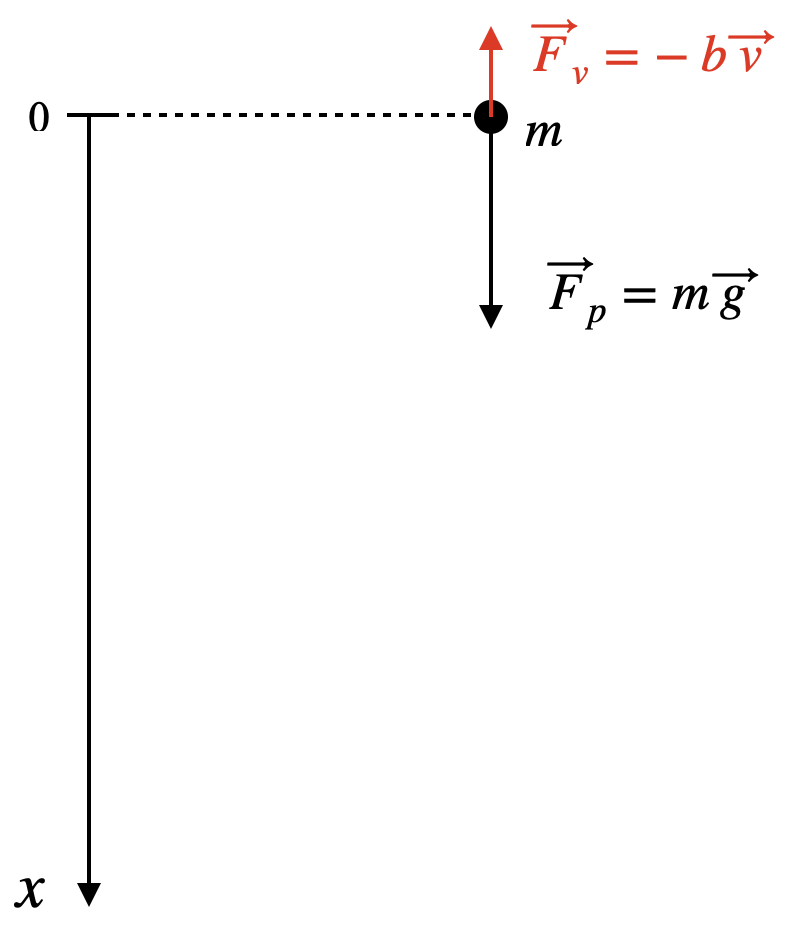
\includegraphics[width=7cm]{images/cadlibera.png}
\caption{Corpo di massa $m$ soggetto alla forza peso ed alla forza di attrito viscoso.}
\label{default}
\end{center}
\end{figure}

Quindi scrivendo la somma delle forze che agiscono su $m$ otterremo:

\begin{equation}
mg - bv = m\dot v \seg \dot v = g - \frac{b}{m}v
\end{equation}
Ora definiamo un tempo caratteristico del sistema, che chiameremo $\tau$. Questo fattore determina una scala temporale del moto. La regione in cui $t\gg\tau$ è chiamata regime, mentre la zona in cui $t\gg\tau$ è chiamata transiente.

\begin{equation}
\boxed{\tau \coloneqq \frac{m}{b} = \frac1\beta}
\end{equation}
Andiamo ora a ricavare la velocità in funzione del tempo.

\begin{equation}
\dot v = g - \frac bmv = g - \frac v\tau = -\frac1\tau\sx v - g\tau\dx\seg \frac{\dot v}{v -g\tau} = -\frac1\tau
\end{equation}

\begin{equation}
\int_0^{v_{(t)}}\frac{d v}{v -g\tau} = -\int_0^t\frac{dt'}\tau\seg \ln\sss 1 - \frac{v_{(t)}}{g\tau}\ddd = -\frac t\tau\seg\boxed{v_{(t)} = g\tau\sx1-e^{-\frac t\tau}\dx}
\end{equation}

Integrando nuovamente si ottiene l'equazione del moto:

\begin{equation}
x_{(t)} = g\tau\int_0^tdt'\sx1-e^{\frac{-t'}\tau}\dx \seg\boxed{x_{(t)} = g\tau\sss t + \tau\sx e^{-\frac t\tau} - 1\dx\ddd}
\end{equation}

\begin{figure}[htbp]
\begin{center}
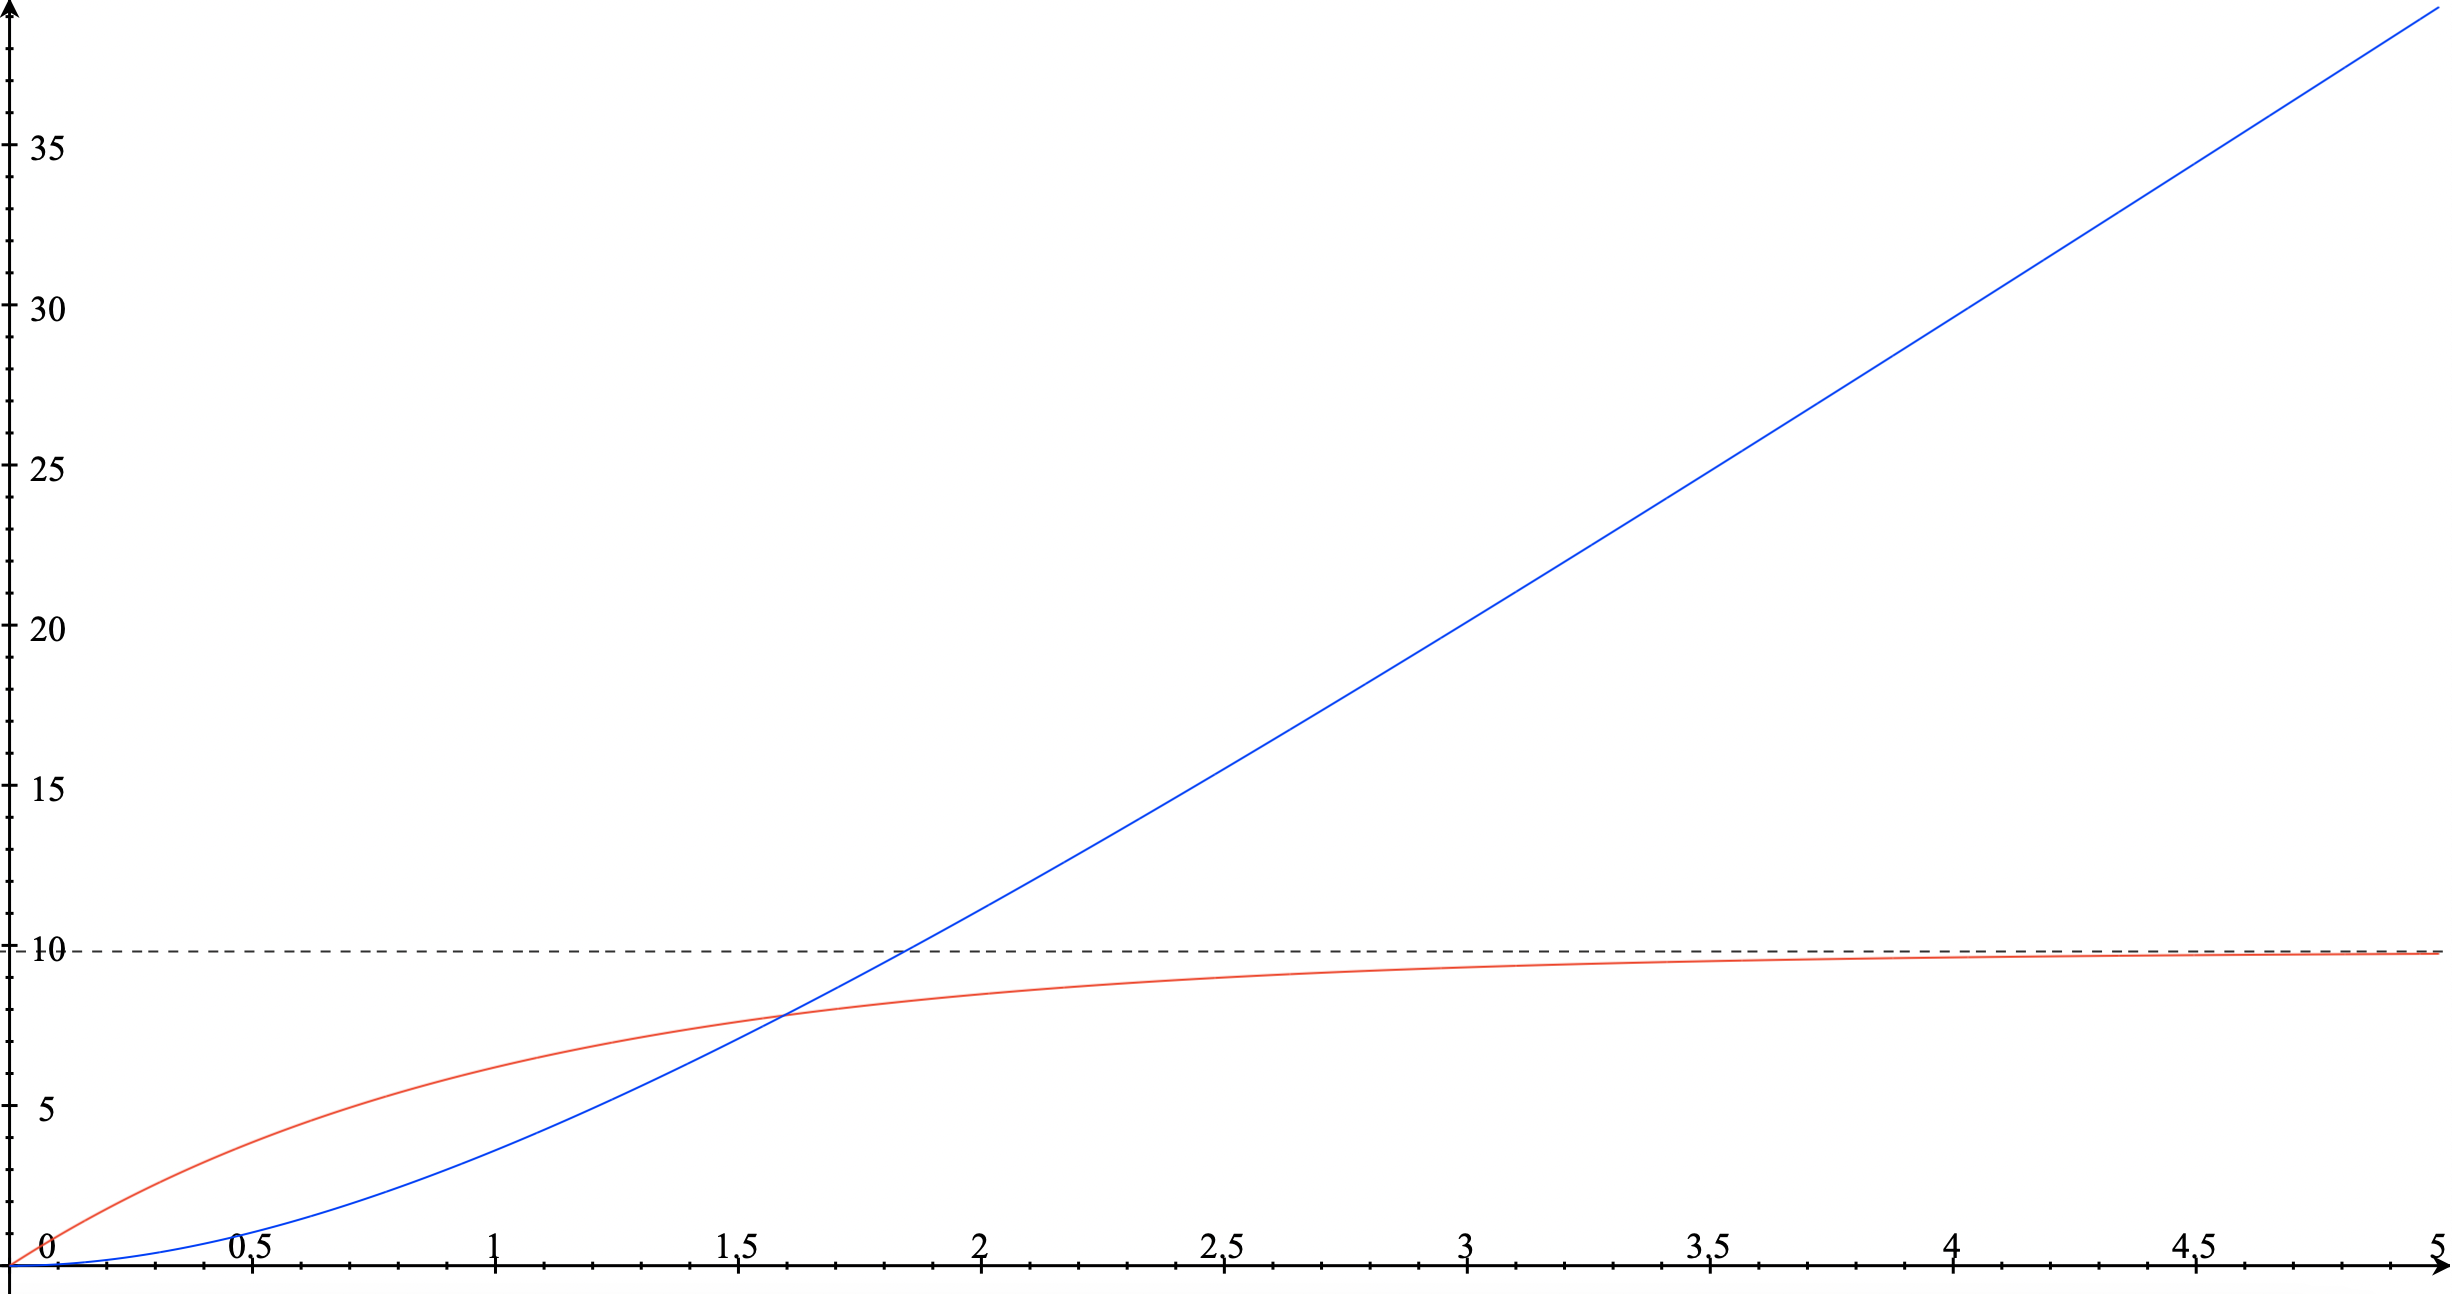
\includegraphics[width=10cm]{images/cadsmorzxv.png}
\caption{Spazio percorso (blu) e velocità (rosso) di un corpo in caduta libera con attrito viscoso. La linea orizzontale tratteggiata rappresenta il valore asintotico (a regime) della velocità. L'asse delle ascisse rappresenta il tempo in unità di $\tau$.}
\label{default}
\end{center}
\end{figure}

Il valore a regime di $v_{(t)}$ si calcola facendo il limite per $t\gg\tau\seg$

\begin{equation}
v_\infty\coloneqq v_{\sx t\gg\tau \dx} = g\tau
\end{equation}

La velocità tende a diventare costante in quanto la forza d'attrito tende a bilanciare la forza peso dunque il corpo tenderà a muoversi di moto rettilineo uniforme.\\
Se invece sviluppiamo sia $x_{(t)}$ che $v_{(t)}$ per $t\ll\tau$, possiamo osservare che l'effetto della forza d'attrito è ancora troppo piccolo e quindi le curve posso essere approssimate con le equazioni della caduta libera senza attrito.

\begin{figure}[htbp]
\begin{center}
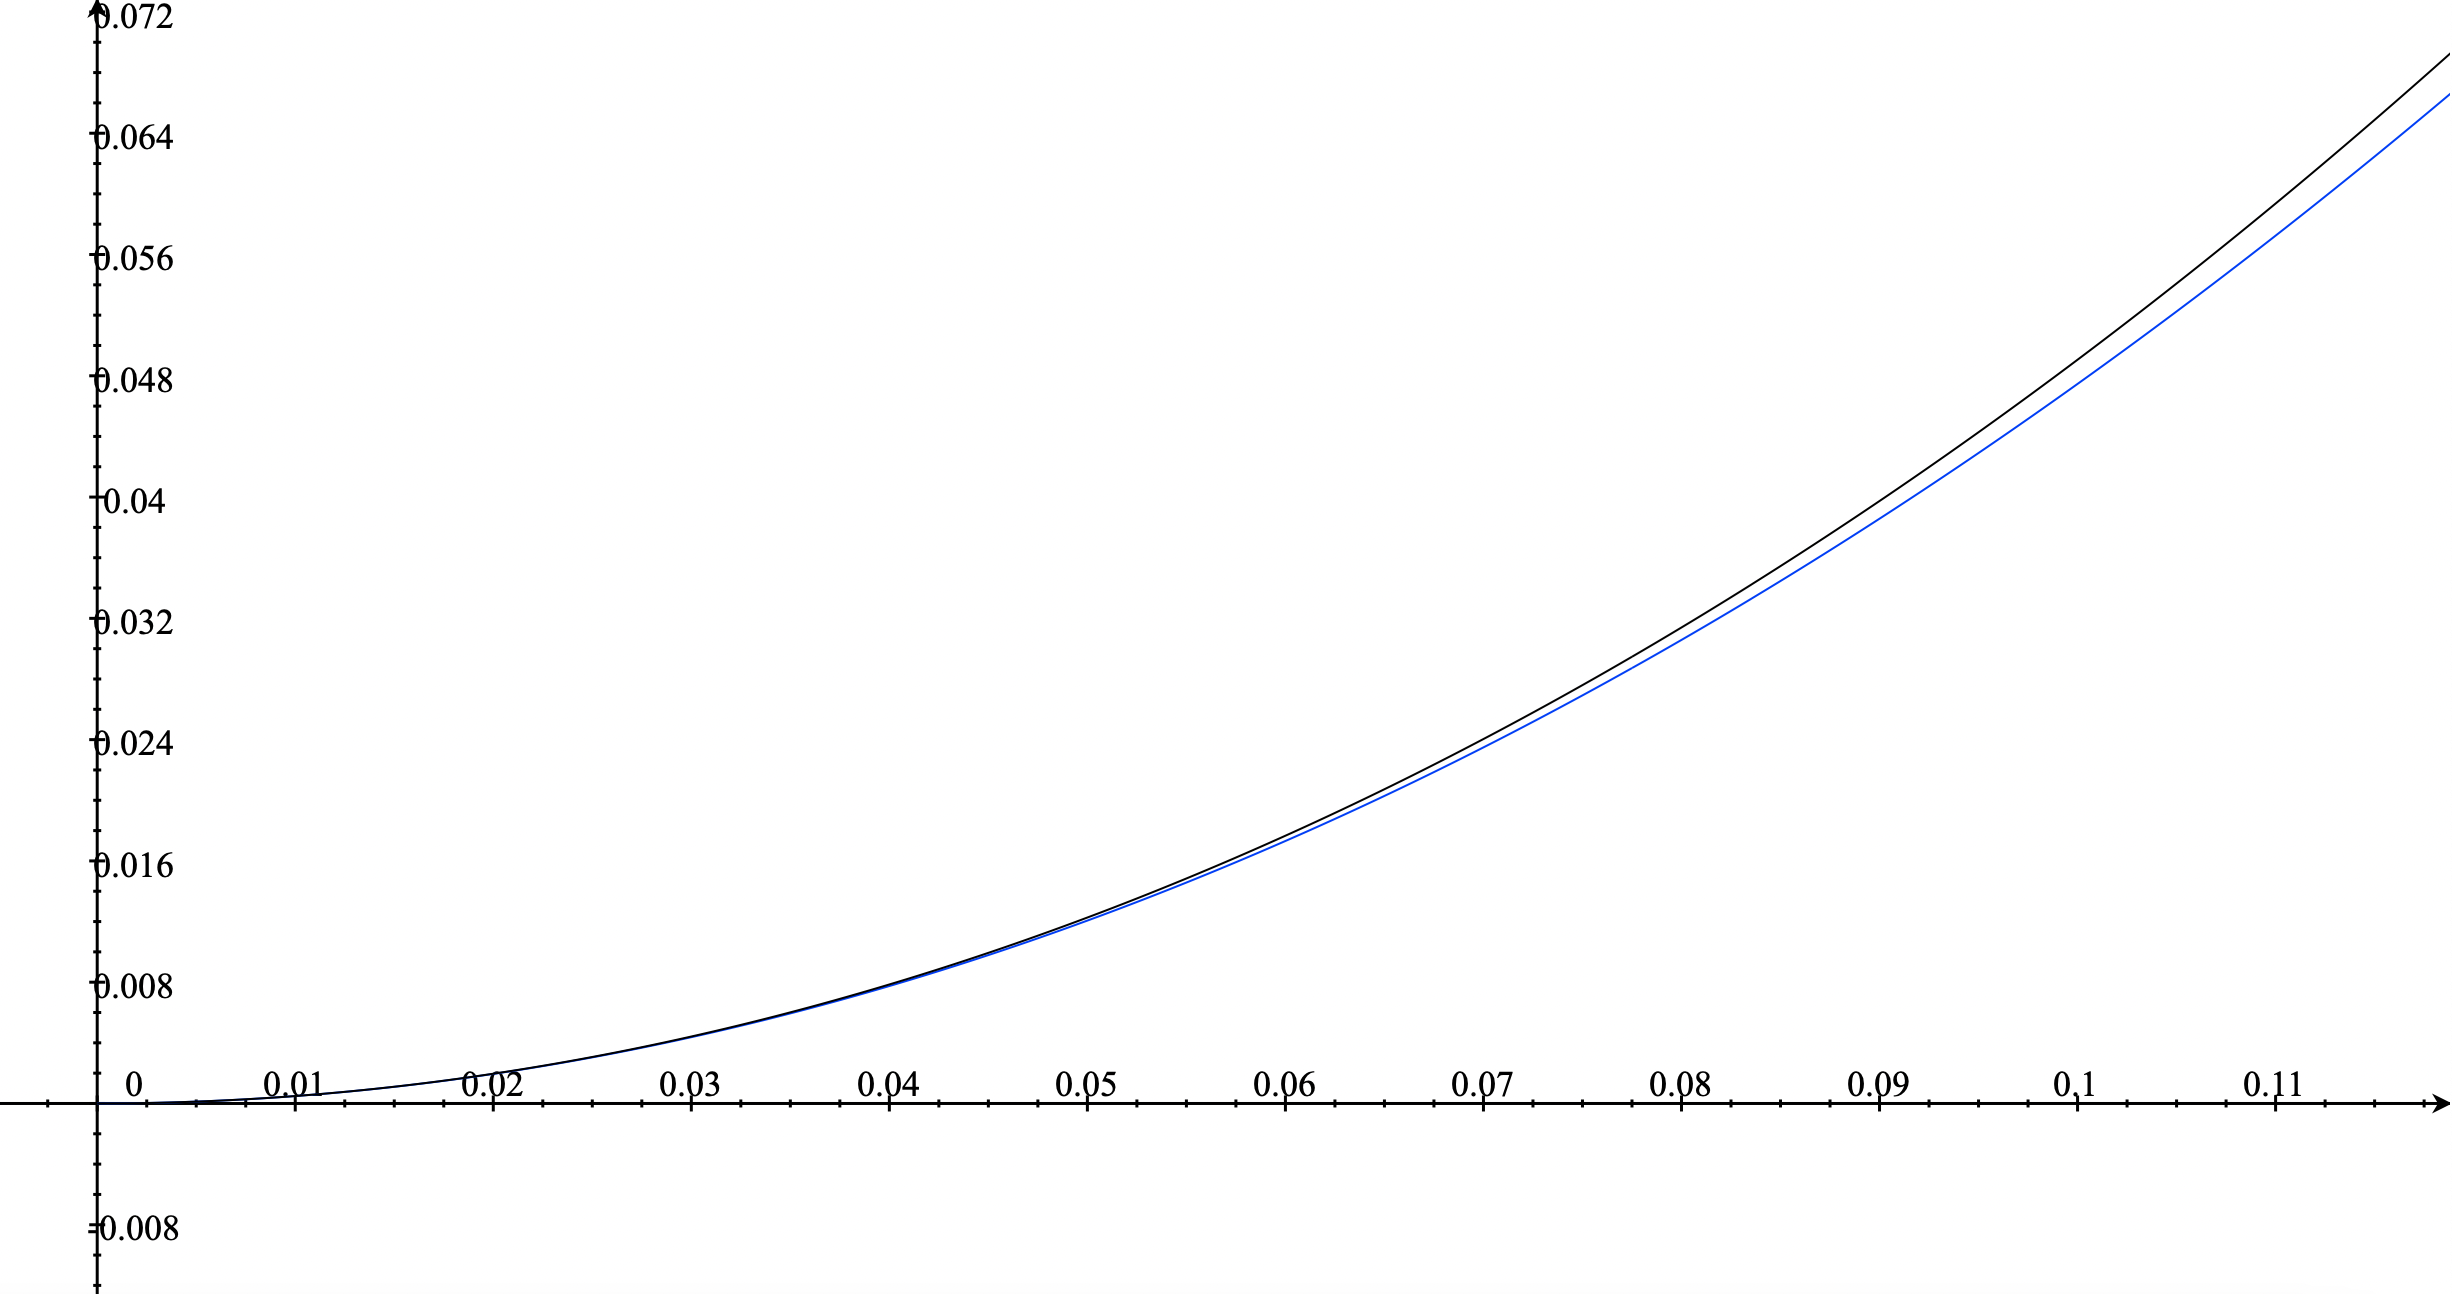
\includegraphics[width=10cm]{images/cadsmorzx.png}
\caption{Approssimazione per piccoli tempi, la curva nera è l'equazione della posizione in funzione del tempo in caduta libera senza attrito: $x_{(t)} = \frac12gt^2$}
\label{default}
\end{center}
\end{figure}

\begin{figure}[htbp]
\begin{center}
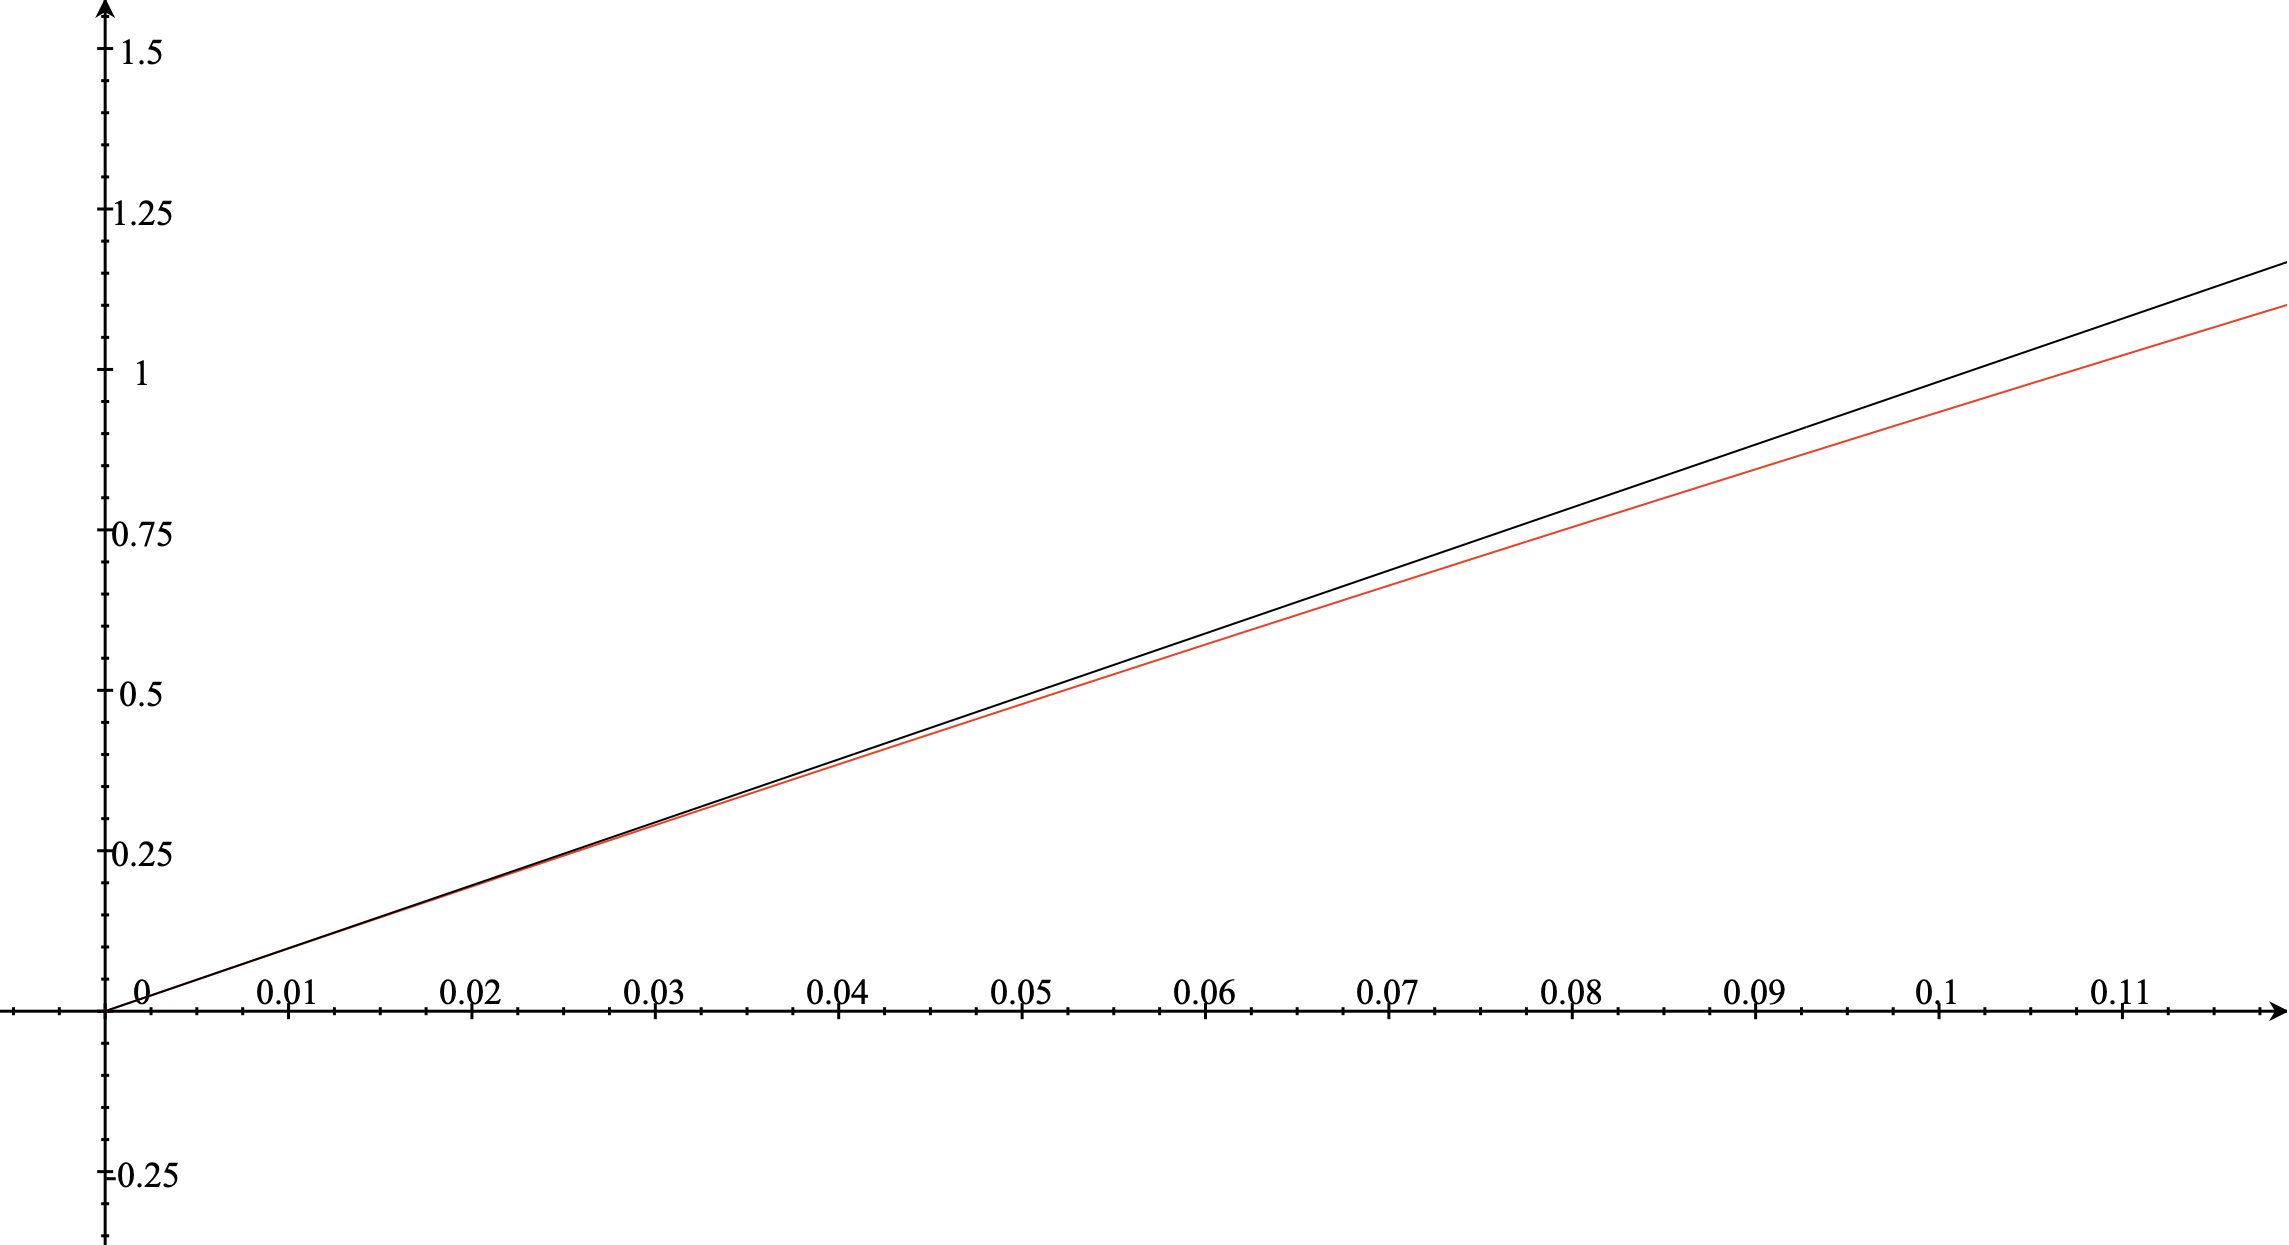
\includegraphics[width=10cm]{images/cadsmorzv.png}
\caption{Approssimazione per piccoli tempi, la curva nera è l'equazione della velocità in funzione del tempo in caduta libera senza attrito: $v_{(t)} = gt$}
\label{default}
\end{center}
\end{figure}

\section{Piano inclinato}
Vogliamo studiare il problema di un punto materiale di massa $m$ in caduta libera, lungo un piano inclinato con pendenza $\theta$. Studieremo prima il caso senza attrito e poi il caso con attrito, trascureremo in entrambi i casi l'attrito viscoso con l'aria. \\
Scegliamo un sistema di riferimento con l'asse $x$ parallelo al piano e l'asse ortogonale ad esso, come mostrato in figura $(2.7)$.
\\ Nel caso senza attrito le forze in gioco sono: la forza peso diretta in direzione verticale e scomponibile in $\vec F_{px}$ ed $\vec F_{py}$, e la forza di reazione vincolare diretta lungo la direzione positiva dell'asse $y$. Dunque avremo che:

\begin{equation}
x:\quad mg\sin\theta = m\ddot x\quad\quad y: \quad N - mg\cos\theta = 0
\end{equation}
$$\Downarrow$$
\begin{equation}
\begin{cases}
a_x = g\sin\theta\\
N = mg\cos\theta
\end{cases}\seg x_{(t)} = \frac12 g\sin\theta\cdot t^2
\end{equation}
Si ha un moto uniformemente accelerato con accelerazione $g\sin\theta$.

\begin{figure}[htbp]
\begin{center}
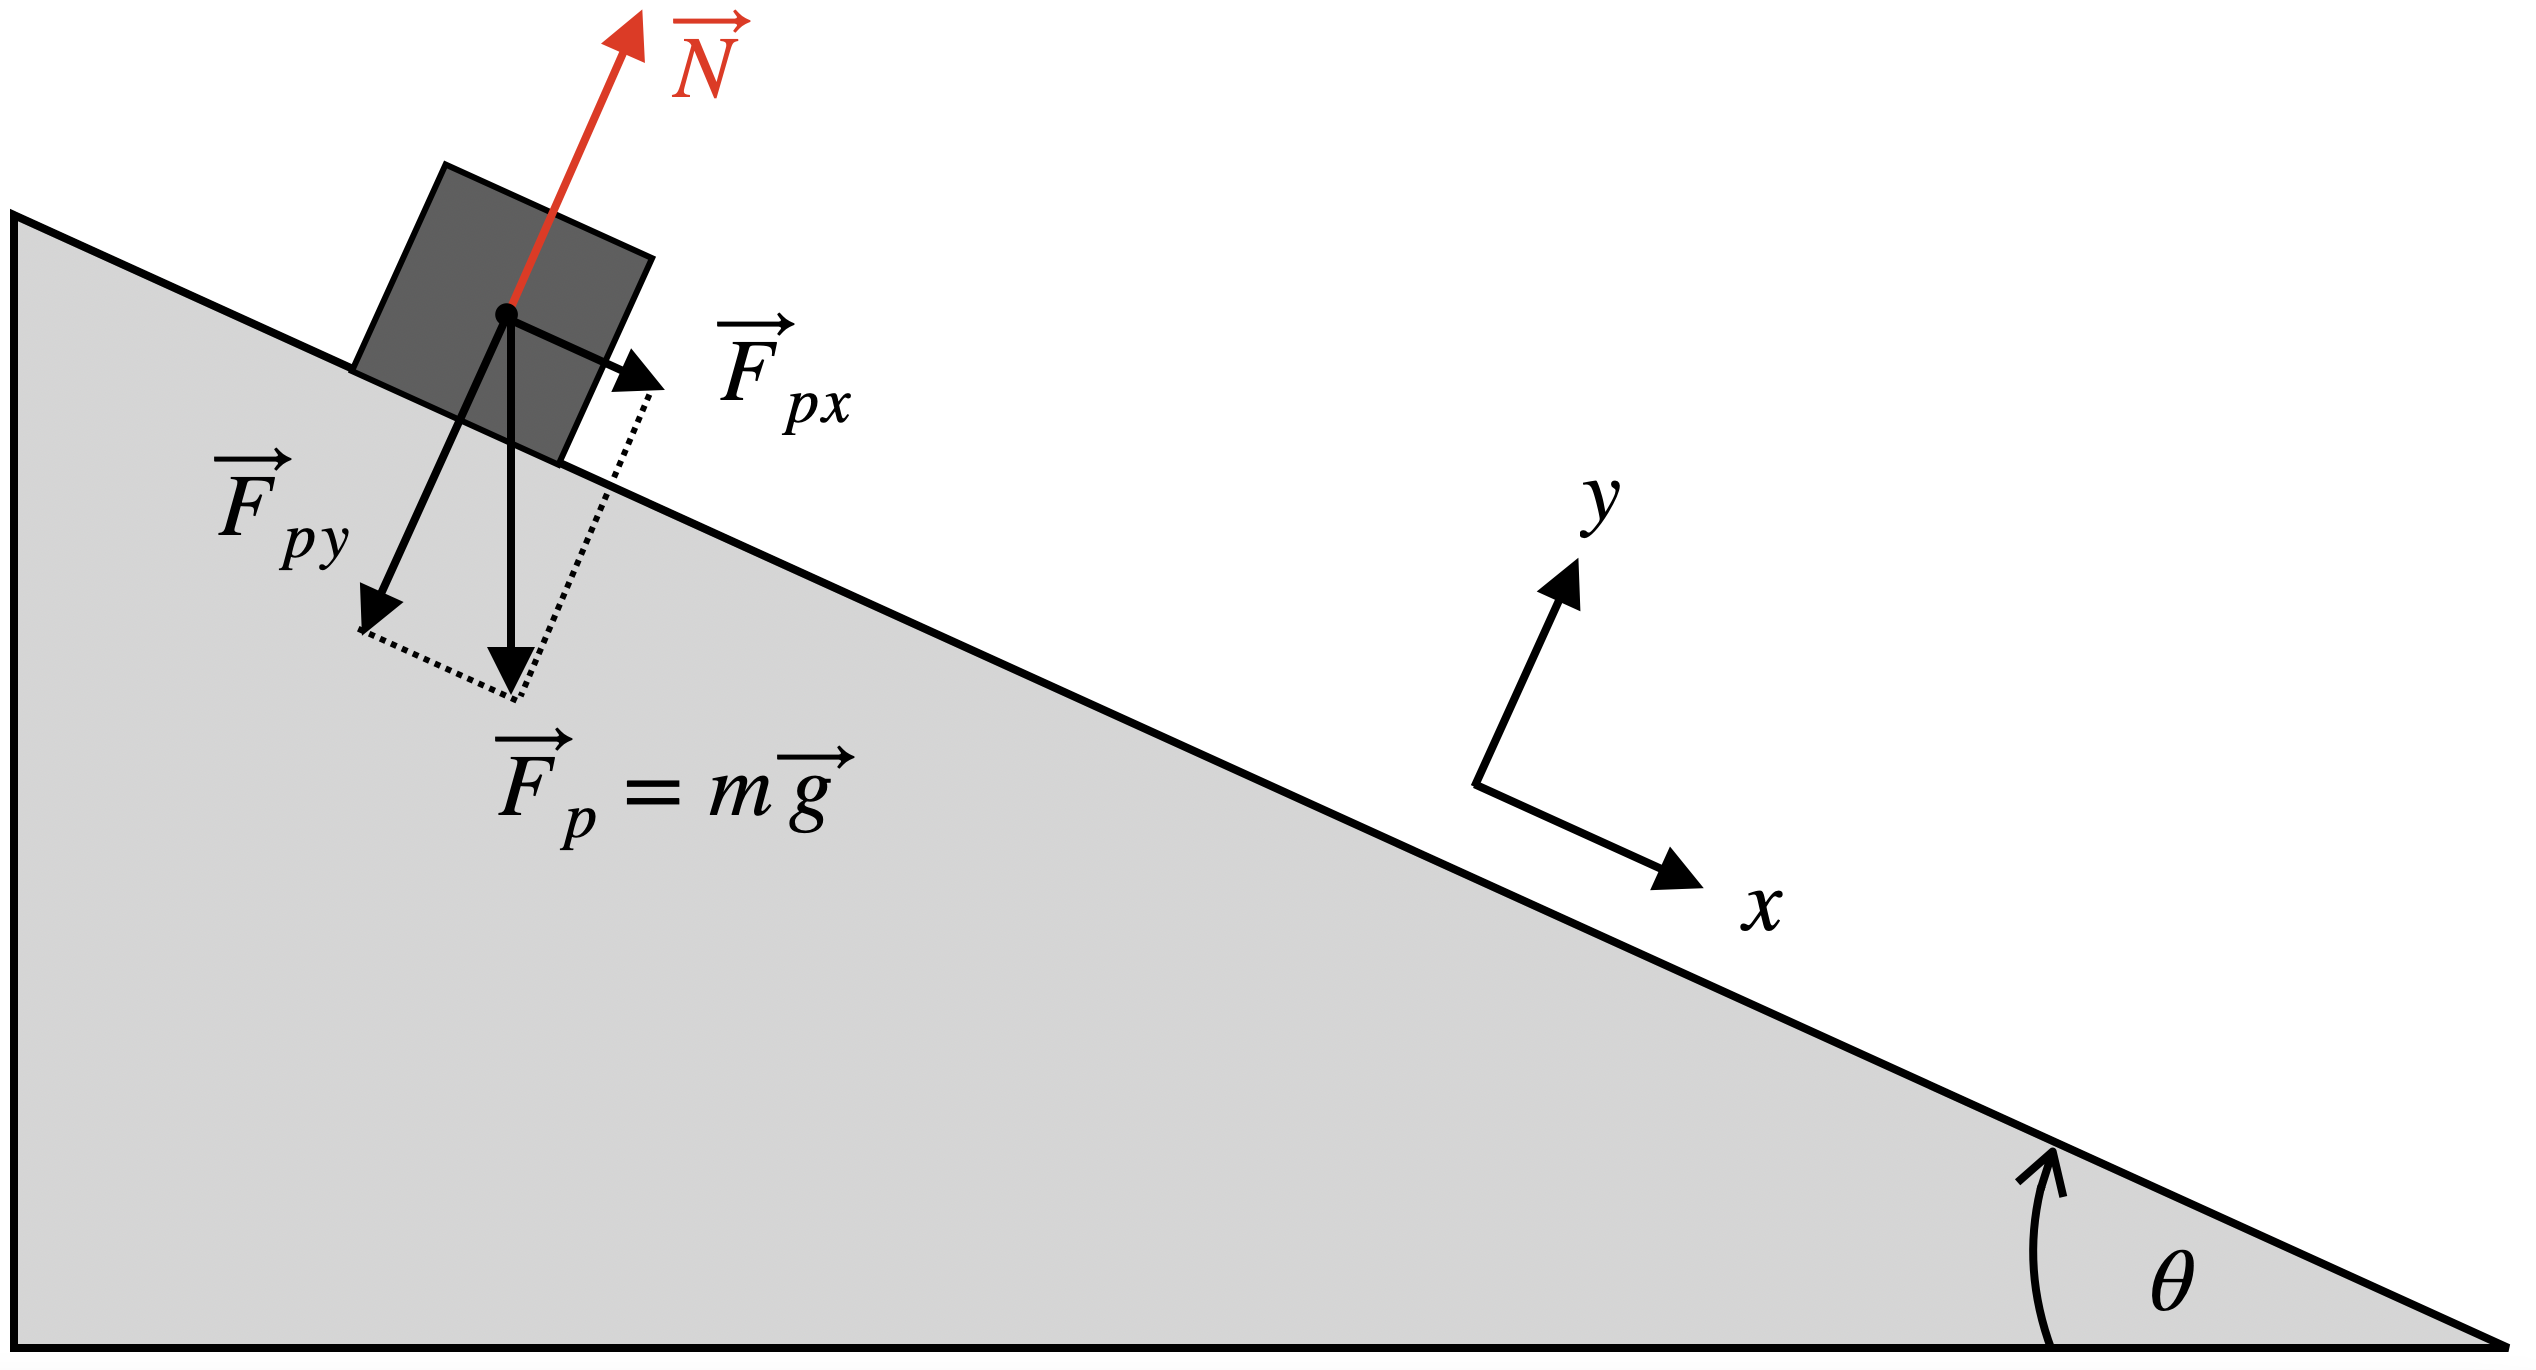
\includegraphics[width=10cm]{images/pianoincl.png}
\caption{Rappresentazione di un piano inclinato con angolo $\theta$ e rappresentazione del sistema di riferimento scelto, con la coordinata $x$ parallela al piano e la $y$ ortogonale.}
\label{default}
\end{center}
\end{figure}

Nel caso con attrito avremo un moto solo se la componente parallela della forza peso è maggiore della forza d'attrito massima:

\begin{equation}
mg\sin\theta > \mu_s mg\cos\theta\seg \boxed{\tan\theta>\mu_s}
\end{equation}

Supponendo di trovarci in questa situazione, studiamo il caso dinamico:

\begin{equation}
x:\quad mg\sin\theta -\mu_d mg\cos\theta = m\ddot x\seg \boxed{a_x = g\sx\sin\theta-\mu_d\cos\theta\dx}
\end{equation}

Dato che $\mu_d<\mu_s$, non può verificarsi il caso in cui $\tan\theta =\mu_d$ che annullerebbe l'accelerazione lungo $x$.




\section{Forza elastica}
La forza elastica è una forza di richiamo generata da una molla, quando viene discostata dalla sua posizione di equilibrio. Essa è proporzionale alla contrazione/dilatazione effettuata.\\ Quindi se supponiamo di avere un un punto collegato ad una molla in posizione iniziale $\vec x_0$, e lo spostiamo fino al punto $\vec x$, allora la forza elastica sarà:

\begin{equation}
\vec F_e = -k\sx\vec x-\vec x_0\dx = -k\Delta x\cdot\hat u_x
\end{equation}

\begin{figure}[htbp]
\begin{center}
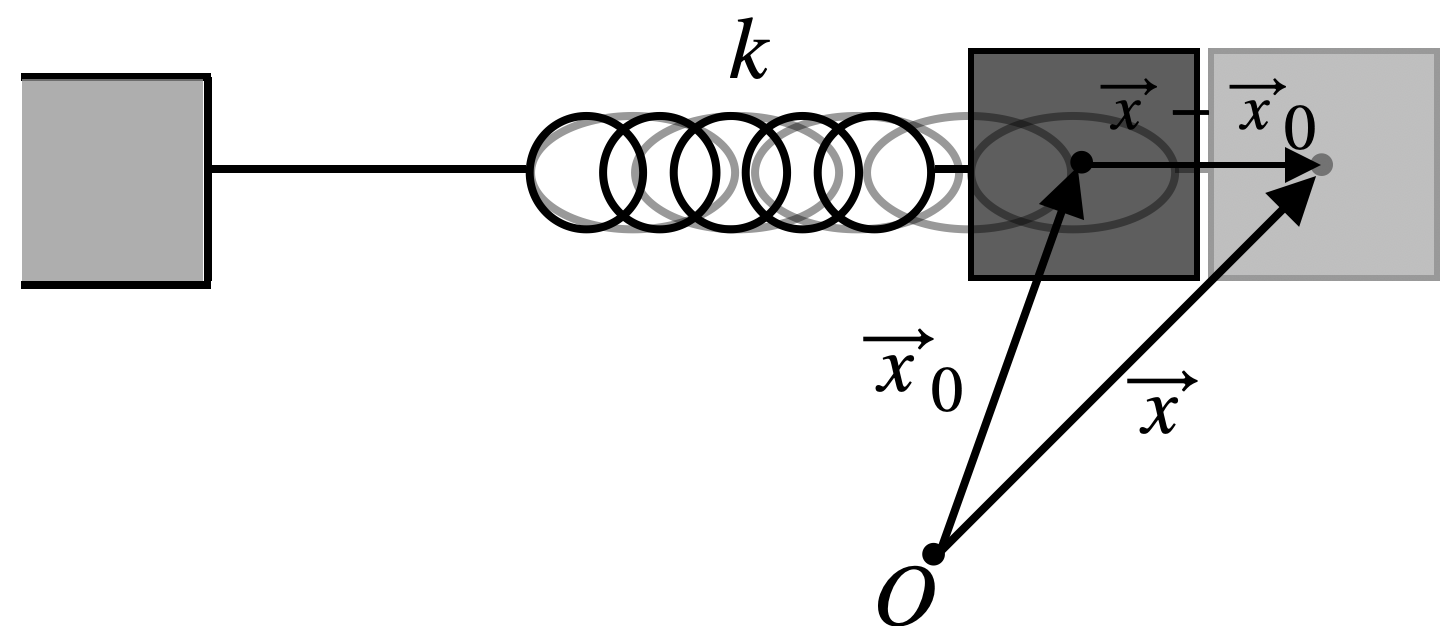
\includegraphics[width=10cm]{images/molla.png}
\caption{Rappresentazione dell'elongazione di una molla rispetto alla sua posizione di riposo.}
\label{default}
\end{center}
\end{figure}

La costante elastica $k$ è caratteristica della molla ed è misurata in $\frac Nm$. Se studiamo il caso dinamico in cui un corpo è soggetto alla sola forza elastica otterremo che:

\begin{equation}
F_x = m\ddot x = -kx \seg \boxed{\ddot x +\frac km x = 0}
\end{equation}

È l'equazione differenziale dell'oscillatore armonico con $\omega = \sqrt{\frac km}$ e periodo $T =2\pi\sqrt{\frac mk}$.
La soluzione sarà come la $(1.7)$, possiamo utilizzare la funzione coseno in quanto il punto parte da una posizione pari a $\Delta x$:

\begin{equation}
x_{(t)} = \Delta x \cos\sx \sqrt{\frac km}t\dx
\end{equation}
In realtà non è necessaria la presenza di una molla per avere una forza elastica, e quindi questo tipo di moto, ma qualsiasi sistema fisico in cui è presente una forza come quella in $(2.35)$ è riconducibile ad un oscillatore armonico semplice.




\section{Pendolo semplice}
\begin{figure}[htbp]
\begin{center}
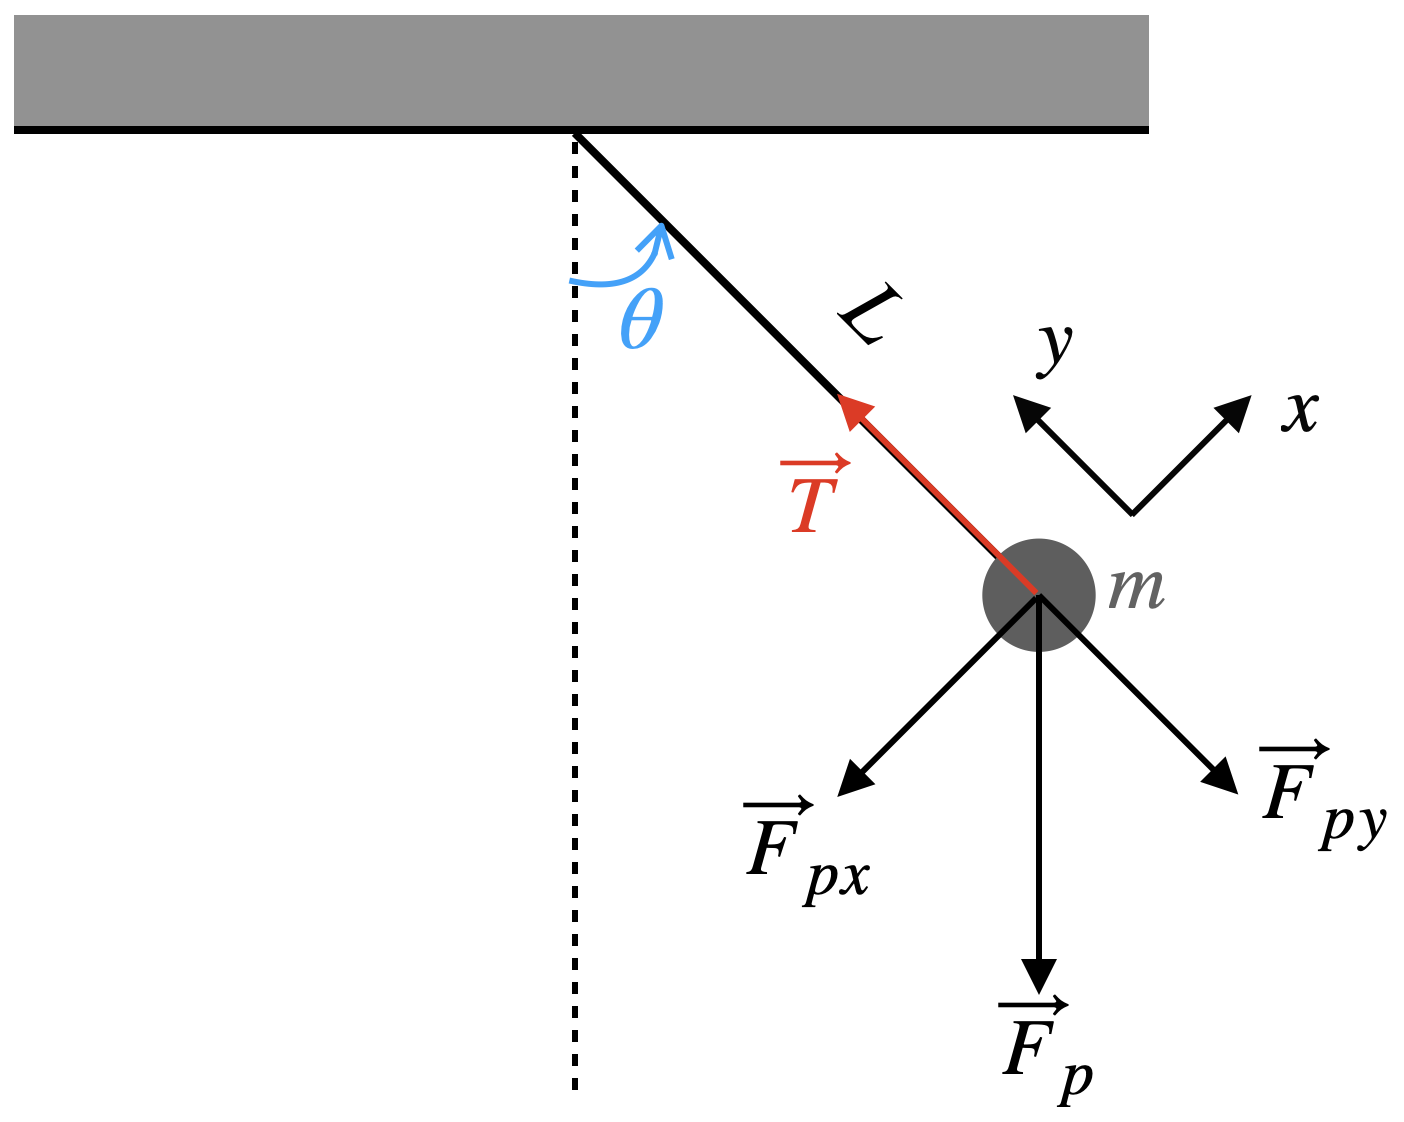
\includegraphics[width=10cm]{images/pendolo.png}
\caption{Rappresentazione di un pendolo inclinato di un certo angolo $\theta$ rispetto alla verticale. È stato raffigurato anche il sistema di riferimento, con l'asse $y$ parallelo al filo di lunghezza $L$, e l'asse $x$ ortogonale ad esso.}
\label{default}
\end{center}
\end{figure}



Il pendolo è un sistema fisico costituito da un punto materiale di massa $(m)$ sottoposto ad una forza costante, in questo caso la gravità, vincolato ad avere una certa distanza $(L)$ da un punto fisso.\\ Nel caso mostrato in figura $(2.9)$, la distanza viene vincolata con un filo inestensibile teso con una tensione $(\vec T)$. Volgiamo studiare la legge oraria dell'angolo $\theta$, l'angolo tra l'asse verticale e la fune.\\ Scriviamo dunque le equazioni di Newton nel sistema di riferimento mostrato in figura $(2.9)$, con un asse parallelo alla fune ed uno ortogonale.

\begin{equation}
x:\quad -mg\sin\theta = ma_t\quad\quad y:\quad T-mg\cos\theta = ma_n
\end{equation}

\begin{equation}
a_t = \frac{dv}{dt}=\frac d{dt}\sx L\dot\theta\dx=L\ddot\theta\quad\quad a_n = 0
\end{equation}
Lungo l'asse $y$ il corpo è in equilibrio, mentre lungo l'asse $x$ abbiamo la seguente equazione differenziale:

\begin{equation}
\boxed{\ddot\theta + \frac gL\sin\theta = 0}
\end{equation}
Se consideriamo l'approssimazione di piccole oscillazioni, l'equazione differenziale appena ottenuta si riduce all'equazione dell'oscillatore armonico, in quanto:

\begin{equation}
\theta \ll 1 \seg \sin\theta \sim \theta \seg \ddot\theta + \frac gL\theta = 0
\end{equation}
Dove la la pulsazione propria del sistema è $\omega_0 = \sqrt{\frac gL}$.
\begin{equation}
\theta_{(t)} = \theta_0\sin\sx\omega_0t+\phi\dx\quad\quad \omega_{(t)} = \omega_0\theta_0\cos\sx\omega_0t+\phi\dx\quad\quad \theta_{(t)} =-\omega_0^2 \theta_0\sin\sx\omega_0t+\phi\dx
\end{equation}